







This chapter is organized as follows.  In Section \ref{themodel}, we describe dynamics  involved for the $k$-species PDMP, including the weights and rules for determining transition probabilities.  In Section \ref{itsapdmp}, we show that the $k$-species PDMP is, in fact, a PDMP by defining the parameters of a general PDMP to align with the model. The main theorem involving a fluid limit for empirical particle densities is then established.
   
Unfortunately, while the PDMP described in Section \ref{itsapdmp} is perfectly well-defined, the set of non-trivial functionals in the domain of its associated generator is too small to describe individual species densities. Section \ref{extension} addresses this issue by adding variables to the original $k$-species PDMP. These extra variables do not interact with the dynamics of the original stochastic process, but rather are simply meant to track certain types of jumping events that occur. With these added dimensions, we are able to produce   martingales, via Dynkin's formula, that serve as estimates of the fluid limit.

The main technical details of existence of limiting densities are provided in Section \ref{cogito}.  The main idea is to differentiate particles according to their paths of visiting differing species, and show empirical measures of certain paths  satisfy tightness conditions. Section \ref{bounddim} gives a law of large numbers argument to establish convergence of terms in the martingale equation.  Finally, Section \ref{cogitotime} shows that existence can be established on a reasonable time interval in the sense that there solutions are well defined as each species has positive total number.          


\section{Notation}

\begin{longtable}[l]{p{50pt}  p{300pt}} \textbf{Symbol}   & \textbf{Description} \\ $\tilde{\mathscr A}_{j,k}^N(t)$    & Boundary running measure of subparticle process $\mathscr A_{j}^N(t)$\\  
 $\tilde{\mathscr A}_{j,k}^{int,N}(t)$    & Interior running measure of subparticle process $\mathscr A_{j}^N(t)$\\ 
$\beta$ & Poisson parameter for interior events\\
$B_{j,k}^{\phi,N}(t)$ & Tracking dimension of particles reassignments from $L_j$ to $L_k$\\
$C_b(\mathbb{R}^+)$ & The space of bounded continuous functions on $\mathbb R^+$\\
$\mathcal C$ & The space of test functions \\
$\Delta X(t)$         & The infinitesimal change of a stochastic process at time $t$\\
 $F_l(t)$ & total number deleted at species $l$\\
$g_k(t)$ & Total total number of species $k$ limit\\
$g_k^0$ & Total initial total number of species $k$ limit\\
$g_k^N(t)$ & Total total number of species $k$ of $X^N(t)$\\
$G(s)$ & Total total number of species $k$ limit\\
$G^{int}(s)$ & Weighted interior total total number of species $k$ limit\\
$H^N(t)$ & The total deleted total number of $X^N(t)$ \\
$K^{(l)}$ & Number of particles reassigned from a boundary event\\ 
$K^{int}$ & Number of particles reassigned from an interior event\\ 
$K$ & $\max_l K^{(l)} \vee K^{int}$\\
$\kappa(t)$ & The total number of particle reassignments before time $t$\\
$\kappa_{j,k}(t)$ & The total number of particle reassignments that send a particle from $L_j$ to $L_k$ before time $t$\\
$L_{i}$    & Species type $i$ \\
$|L_{i}|$    & Number of particles of species type $i$ \\
$m(t)$ & The total number of critical events before time $t$\\
$m_{int}(t)$ & The total number of interior events before time $t$ \\
 $M$ & The number of  different species\\
  $(\mathfrak M,d)$ & A metric space $\mathfrak M$ with distance $d$\\
  $M_-$ & The number of  species with negative velocities\\
 $M_0$ & The number of  species with zero velocities\\
 $M_+$ & The number of  species with positive velocities\\
 $\mu^N_k(t)$ & Empirical measures of species $k$ of $X^N(t)$ \\
$\mu^N_\Sigma(t)$ & Path measures of $X^N(t)$ for path $\Sigma$ \\
$\mu_k(t)$ & Limiting empirical measures of species $k$\\
$\mu_k^0$ & Limiting initial empirical measures of species $k$\\
 $N(t)$    & Number of particles at time $t$\\
 $N^{(l)}$ & Species selection numbers for boundary events\\
$N^{int}$ & Species selection numbers for interior events\\
$p_i^{(l)}$ & Species selection probabilities for boundary events\\
$p_i^{int}$ & Species selection probabilities for interior events\\
$\varphi^i(x,t)$ & Flows corresponding to $v_i(x)$\\
$\mathscr P(x(t))$ & Path of a particle\\
$R_{ij}^{(l)}$ & Reassignments for boundary events\\
$R_{ij}^{(l)}$ & Reassignments for interior events\\
$S_i(\mathbf x)$ & Support of particles in species $i$\\
$\Sigma(x(t))$ & Path location of a particle\\
$T_e$ & Length of existence interval\\
$\tau_i(t)$ & The $i^{th}$ jump time of a critical event.\\
$\tau_i^{j,k}$ & The time of the $i^{th}$ occurrence of a boundary event reassignment  that sends a particle from $L_j$ to $L_k$.\\
$\Theta(x(t))$ & Jump description of a particle\\
$u_k(x,t)$ & Smooth density limit of species $k$\\
$v_{i}(x)$ & The velocity at $x \in L_i$\\
$w_{i}^{(l)}$ & Species selection weights for boundary events \\
$w_{i}^{int}$ & Species selection weights for interior events \\
$W_{j}^{(l)}$ & Species selection weight fraction for boundary events of species $k$ limit\\
$X^N(t)$ & The $k$-species PDMP with $N$ initial particles\\
$\tilde X^N(t)$ & The $k$-species extended PDMP with $N$ initial particles

\end{longtable}  
\section{A kinetic mixing model}\label{themodel}
\subsection{The model}
Our PDMP for particle evolution tracks $N(t)$ particles $X(t) = (x_1(t),\dots x_N(t))$, with $N(0) = N$,  on disjoint species $L_i = \mathbb{R}^+_i, i = 1, \dots, M$.   A species $L_i$ is equipped with a vector field $v_i(x)\in C^1(\mathbb{R}^+)$, where $v_i$ is strictly positive, strictly negative, or identically zero.  The vectors fields are also assumed to define flows $\varphi^i(x,t)$ with no finite time blowup.  We write  $M = M_-+M_0+M_+$, representing species with positive, stationary, and negative velocity, respectively. Specifically for $i = 1, \dots, M_{1}$ we equip $L_i$  with vector fields  $v_i<0$, while for $i = M_-+1, \dots, M_-+M_0$, $v_i \equiv 0$, and for $i = M_-+M_0+1, \dots, M$, $v_i > 0$.   Particles move according to $\varphi^i(x,t)$ until one of the following two \textbf{critical events} occur:\begin{enumerate}
\item 
\textbf{Boundary event:} A particle $x_j(t) \in \mathbb{R}^+_i, i \in 1, \dots M_-$ hits the origin.
\item
\textbf{Interior event:} A Poisson clock with a parameter rings.
\end{enumerate} 
When a critical event occurs, particles can either be instantly deleted or transferred to another species.  However, no spatial jumps occur, meaning that critical events do not change the position of particles.  A particle $x_i(t) \in L_j$ that reaches 0 is instantly deleted.

 

 
  

We use mean field probabilities to determine where particles are reassigned at a critical event. At a boundary event triggered by a particle hitting the origin of $L_l$, $K^{(l)}$ species are randomly selected according to constants $w^{(l)}_i \ge 0$, $i = 1, \dots, M$, and  a probability vector $p^{(l)}(w^{(l)}_1, \dots,w^{(l)}_M)$, where 
\begin{equation}
p^{(l)}_i = \frac{w^{(l)}_i |L_i|}{ N^{(l)}},   \quad N^{(l)} = \sum_{j = 1}^M w^{(l)}_j |L_j| \quad i = 1, \dots, M.
\end{equation}
 Note that $p_i^{(l)}\ge0$, and $\sum_{i=1}^M p_i^{(l)}= 1$.
When a species $L_i$ is chosen, one particle is then selected with equal probability $1/|L_i|$ from particles in $L_i$.  The selected particles $x_{1}, \dots, x_{K^{(l)}}$ will be reassigned to a new species according to a reassignment $R^{(l)}_{ij}\in \{1, \dots, M\}$, with $i =1, \dots, M,j = 1, \dots, K^{(l)}$.  Explicitly, if a particle $x_j$ is in $L_i$, then after its jump, it is assigned to $L_{R^{(l)}_{ij}}$. We stress the importance of the $j$ parameter in $R_{ij}^{(l)}$, since it means that the order a particle is chosen at a critical event can affect its reassignment.  For interior events, we select $K^{int}$ particles according to a probability vector $p^{int} =  (w^{int}_1, \dots,w^{int}_M)$, with $w_i^{int} \ge 0$ and
\begin{equation}
p^{(l)}_i = \frac{w^{int}_i |L_i|}{ N^{int}},   \quad N^{int} = \sum_{i = 1}^M w^{int}_i |L_i|.
\end{equation}
 Particles are  reassigned according to $R^{int}_{ij}\in\{1, \dots, M\} $. After jumps occur, particles continue to drift along flow lines as before until another critical event occurs. See Fig. \ref{pdmppic} for an example on four species. 


\begin{figure}
\begin{centering}
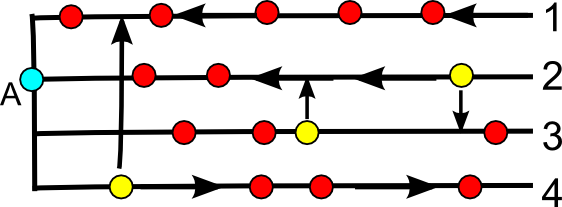
\includegraphics[width=.5\textwidth]{gen_pdmppic.png}
\caption{\textbf{A PDMP on four species}.  Particles travel on four separate copies of $\mathbb{R}^+$.  Velocity directions are represented by horizontal arrows, with species 3 having zero velocity. A boundary event occurs when a particle (labelled by ``A") hits the origin.  Here, three particles  are then randomly selected ($K^{(2)} = 3$), and reassigned  to different species by predetermined reassignments (given by vertical arrows). In this example, $R_{41}^{(2)} = 1, R_{32}^{(2)} = 2$, and $R_{23}^{(2)} = 3$. }
\label{pdmppic}
\end{centering}

\end{figure}  





 













\section{The $k$-species model in a PDMP framework}\label{itsapdmp}
\subsection{PDMP formulation of  the $k$-species model} 
We now show the $k$-species model is a specific class of PDMP, as outlined in Section \ref{pdmpgenerator}. Define the possible listings of species
\begin{equation}
 \mathcal S= \bigcup_{i \in \mathbb N}\{1, \dots, M\}^{i},
 \end{equation}   For a species index $\mathbf { s} = (s_{1},\dots, s_{|\mathbf s|})$ of length $|\mathbf s|$, a state has the form $(x_1, \dots, x_{|\mathbf s|})\in (\mathbb{R}^+)^{|\mathbf s|}$. 
 We write the state space of particles as    
\begin{equation}
E =\coprod_{\vec s \in \mathcal S } ((\mathbb{R}^+)^{|\mathbf s|})_\mathbf s = \left\{(\textbf s,(x_{1}, \dots, x_{|\mathbf s|}):\textbf s \in \mathcal S, (x_{1}, \dots, x_{|\mathbf s|})\in \mathbb{(R}^+)^{|\mathbf s|}\right\}.  
\end{equation}
A state $\textbf{x} \in E$ can thus be described as an element of  $(\mathbb{R}^+)^{|\mathbf s|}\times \mathbb N^{|\mathbf s|}$, where we will write
\begin{equation}
\textbf{x} = \left((s_{1},x_1), \dots, (s_{|\mathbf s|},x_{|\mathbf s|})\right).
\end{equation} 
Vector fields will then be represented by  
\begin{equation}
\mathcal X_{\vec s} = \sum_{i = 1}^{N} v_{s_i}(x_i)\frac{\partial}{\partial x_i}.
\end{equation}


   The exit boundary of $\Gamma^*\subset E$ consists of  particles that hit the origin.
\begin{equation}
\Gamma^* = \{\mathbf x\in E| \hbox{there exists }  (s_i,x_i) \hbox{ where }   x_i = 0, s_i\le M_-\} 
\end{equation}

To describe the transition kernel $Q$, we denote the set of states that  $\textbf{x} \in \Gamma^*$ can jump to as $E_b(\textbf{x})$.  This set of events is finite, and have well-defined (albeit, tedious to calculate) probabilities of a reassignment for a state $\textbf{x}$ jumping to $\textbf{x}_b$, denoted $p_{b}(\textbf{x}_b, \textbf{x})$.  These probabilities are uniquely determined from the weights $w^{(l)}_k$, numbers $|L_i|$, and reassignments $R_{ij}^{(l)}$, and therefore are functions of the current state $\textbf{x}$.   Similarly, we can define jump probabilities for interior events as $p_{int}(\textbf{x}_{int},\textbf{x}) $. Here, $\textbf{x}_{int} \in E_{int}(\textbf{x})$ denotes the set of possible states that $\textbf{x}\in E$ can jump to.  Thus, we can define
\begin{equation}
Q(y,\textbf{x}) = \begin{cases}p_{b}(y,\textbf{x}) & \textbf{x} \in \Gamma^*, y\in E_b(\textbf{x}) \\
p_{int}(y,\textbf{x}) & \textbf{x} \in E, y \in E_{int}(\textbf{x})   \\
0 & \hbox{otherwise}. 
\end{cases}
\end{equation}
Since each particle has a Poisson clock of parameter $\beta$, the distribution $Y$ of the first time that a clock rings follows the distribution 
\begin{equation}
Y \sim \min_{1\le i\le N} Poisson(\beta) = Poisson(N\beta).
\end{equation}
Thus $\lambda(\textbf{x}): E \rightarrow \mathbb{R}$ takes the form
\begin{equation}
\lambda(\textbf{x}) = \beta |\mathbf s|.
\end{equation}
With this, we now have a well defined PDMP which describes particle reassignments among different species.

\subsection{The main theorem}


For $\textbf{x} \in E$, we define empirical measures $\mu^N_i(\textbf{x}) \in \mathcal M(\mathbb{R}^+)$ by
\begin{equation}
\mu_i^N(\textbf{x}) = \sum_{x_j \in L_i} \frac{\delta_{x_j}}{N}, \quad i = 1,\dots, M.
\end{equation}
For a process $X(t)$, we will often write $\mu_i^N(X(t)):=\mu_i^N(t)$.
For the class of test functions
\begin{equation}
\mathcal C = \{\phi\in C^1(\mathbb{R}^+)\cap C_b(\mathbb{R}^+) : \phi(0) = 0, \phi' \in C_b(\mathbb{R}^+)\},
\end{equation} 
we can pair empirical measures with test functions through integration:
\begin{equation}
\langle \phi, \mu_i^N \rangle = \int_{\mathbb{R}^+} \phi(x)\mu_i^N(dx) = \sum_{x_j \in S_i} \frac{\phi(x_j)}{N}, \quad \phi \in \mathcal C, i = 1, \dots, M,
\end{equation}
where $S_i$ denotes the support of particles in species $i$, for $i = 1,\dots, M$ .

Our main result shows that empirical measures $\mu^N_k(t)$ approximate a weak solution to a transport equation, with a source term given by the flux of particles from both interior and boundary events. These measures are simplest to describe  when viewed as smooth limits $\mu_k(t)$  of particle densities $\mu_k^N(t)$ as $N\rightarrow \infty$ of the form
\begin{equation}
u_k(x,t)dx = \mu_{k}(t)(dx),     \quad k = 1, \dots, M.  
\end{equation}
We also denote the total numbers
\begin{eqnarray}
\lefteqn{g_k(t)= \int_0^\infty u_k(x,t) dx,}\\
&& G(s) = \sum_{i = 1}^M g_i(t), \quad G^{int}(s) = \sum_{i = 1}^Mw_k^{int}g_k(t), \quad k = 1, \dots, M. \nonumber 
 \end{eqnarray}
and species selection weight fractions for boundary events
\begin{equation}\label{sswf}
W_j^{(l)}(t)= \frac{w^{(l)}_j}{\sum w^{(l)}_m g_m(t)} \quad l = 1,\dots, M_{-} \quad j = 1,\dots, M.
\end{equation}
The limiting number densities $u_k(x,t)$, $k = 1, \dots, M$, will satisfy the following system of PDE,
 \begin{eqnarray} 
  \lefteqn{\partial_t u_k(x,t)+\partial_{x}(v_k(x)u_{k}(x,t))=  \phantom{u_j(x,t)\mathbf{1}_{R^{(l)}_{ij}}
-K^{(l)}W_k^{(l)}(t)u_k(x,t)}}\label{smooth1}\\
 && \sum_{l = 1}^{M_-}u_l(0,t)v_{l}(0)\left[\sum_{i = 1}^{M}\sum_{j= 1}^{K^{(l)}} W_i^{(l)}(t)u_i(x,t)\mathbf{1}_{R^{(l)}_{ij}=k}
-K^{(l)}W_k^{(l)}(t)u_k(x,t)\right]\label{smooth2}\\ 
&&+\frac{\beta G(t)}{G^{int}(t)}\left( \sum_{i = 1}^{M}\sum_{j= 1}^{K^{int}} w^{int} _iu_{i}(x,t)\mathbf{1}_{R^{int}_{ij} = k}-K^{int}w^{int}_ku_{k}(x,t)
 \right)\label{smooth3}
 \end{eqnarray}
 with initial conditions 
 \begin{equation}
u_k(x,0) = u_{k}^0(x), \quad k = 1,\dots, M.
\end{equation}

  The first line (\ref{smooth1}) describes advection of species densities under the velocity field $v_k$.  The next line (\ref{smooth2}) describes the  the growth and loss of species $k$ due to boundary events. The first term of  (\ref{smooth2}) describes rates of incoming particles to species $k$.  This is reflected in the use of indicator functions, where  $R_{ij}^{(l)}$ determine species to which particles are reassigned. The next term describes loss from species $k$ to other species. This does not depend on reassignment, so we should expect no $R_{ij}^{(l)}$ terms.      The final line (\ref{smooth3}) contain source terms due to interior events.  These terms do not depend on $u_l(0,t)$, as the rate of interior events is only dependent on total total numbers $g_i(t)$.

  Our main theorem describes the convergence  of empirical measures to a weak form of the limiting PDE (\ref{smooth1})-(\ref{smooth3}), under the assumption of convergence of initial empirical measures to a nonatomic measure. 

\begin{theorem}\label{pdmpproof}
Let $\mu_k^0 \in\mathcal M(\mathbb{R}^+)$ be nonatomic. Suppose that we have weak convergence of initial empirical measures $\mu_k^{0,N} \rightarrow \mu_k^0$ as $N\rightarrow \infty$ in $\mathcal M(\mathbb{R}^+)$.  Then 
\begin{enumerate}
\item There exists a  time $T_e>0$ such that the   $\mu_k^N(t)$ converge to  limits $\mu_k(t)$ along a subsequence under the Skorohod topology $\mathbb D([0,T_e],\mathcal M(\mathbb{R}^+))$.
\item The empirical losses $F_l^N(t)$ of the total number deleted in species $l$  converge to continuous cumulative distribution functions $F_l(t)$ along a subsequence in the mean $L^\infty$ metric:
\begin{equation}
\lim_{N\rightarrow \infty}\mathbb E\left[\sup_{s\le T_e}|F_l^{N}(s)-F_{l}(s)|\right  ]= 0.
\end{equation}
\item The  $\mu_k(t)$ satisfy the following limiting equations for all
$\phi \in \mathcal C:$
\begin{eqnarray}\label{limeq}
\lefteqn{\langle \mu_k(t), \phi\rangle  - \langle \mu_k^0, \phi\rangle+\int_0^t\langle \mu_k(s), \phi' v_k \rangle=}\\ 
&&\sum_{l = 1}^{M_-}\mathlarger{\int_0^t} \left[\sum_{i = 1}^{M}\sum_{j= 1}^{K^{(l)}}W_i^{(l)}(s)\langle \mu_i(s), \phi\rangle\mathbf{1}_{R^{(l)}_{ij} = k}  -K^{(l)}W_k^{(l)}(s)\langle \mu_k(s), \phi\rangle\right ] \, dF_{l}(s)\nonumber\\  
&& +\mathlarger{\int_0^t}\frac{\beta G(s)}{G^{int}(s)}\left[-K^{int}w^{int}_k\langle \mu_k(s), \phi \rangle +\sum_{i = 1}^{M}\sum_{j= 1}^{K^{int}} w^{int}_i\ \langle \mu_i(s), \phi \rangle\mathbf{1}_{R^{int}_{ij} = k}\right]ds, \nonumber
\end{eqnarray}
for $k = 1, \dots, M$.


\end{enumerate}
 


\end{theorem} 
\begin{rem}\label{unifremark}
Since individual jumps of the prelimit PDMP converge to zero as $N\rightarrow \infty$, the limiting functions $\langle \mu_k(t), \phi\rangle, k = 1, \dots, M$ are continuous in $t$, meaning that empirical measures also converge in the local uniform metric (see Prop. 1.17 in Chapter VI of \cite{jac87}).    
\end{rem}
As we will see in Section \ref{bounddim}, the functions $F_l(s)$ can be seen as an integral of the trace of measures $\mu_l(s)$ occurring at the boundary. In fact, for continuous solutions, we will show that $dF_l(s) = v_l(0)u(0,s)ds$. 

We also state a well-posedness theorem for $L^1\cap L^\infty$ initial data, which is proved in Section \ref{uniquesect}.

\begin{deef}
For $k = 1, \dots, M$, let $u_{k}(x,t) \in C([0,T_e],L^1\cap L^\infty(\mathbb{R}^+,\mathbb{R}^+))$. We call $u_{k}(x,t)$ a \textbf{weak solution in $L^1\cap L^\infty(\mathbb{R}^+,\mathbb{R}^+)$} of  (\ref{smooth1}) with initial conditions $u_k^0(x) \in L^1\cap L^\infty(\mathbb{R}^+,\mathbb{R}^+),$ if for all $\phi\in \mathcal C$, there exist $\mu_k(t)$, $t\in [0,T_e]$, that satisfy (\ref{limeq}), with $\mu_k(t)(dx) = u_{k}(x,t)dx$, and $\mu_k(0)(dx) = u_{k}^0(x)dx$.   
\end{deef}

\begin{theorem}\label{wellposed} For $k = 1, \dots, M$,  there exists a unique   weak solution $u_{k}(x,t)$ in $L^1\cap L^\infty(\mathbb{R}^+,\mathbb{R}^+)$ of  (\ref{smooth1}) with initial conditions $u_k^0(x) \in L^1\cap L^\infty(\mathbb{R}^+,\mathbb{R}^+)$.
\end{theorem}

\begin{rem}
Theorem \ref{wellposed} should not be mistaken as stating that empirical measures with $L^1\cap L^\infty$ initial data converge in the uniform metric to a unique $L^1\cap L^\infty$ solution of (\ref{limeq}). Rather, in the class of all possible solutions, there is one, and only one, solution that is in $C([0,T_e],L^1\cap L^\infty(\mathbb R^+))$    \end{rem}
 
Well-posedness of  (\ref{limeq}) for $L^1$ data is discussed in Section \ref{uniquesect}.  




\subsection{Method of proof}


As a Markov process, the PDMP $X(t)$has an associated infinitesimal generator and martingale, given by \ref{generator} and \ref{martingale}, along with Rolski's conditions for membership in the domain $\mathcal D(\mathcal A))$, as shown in Theorem \ref{fourcond}. The method for proving Theorem \ref{pdmpproof} relies on   constructing  martingale equations that are approximations of (\ref{limeq}).  Unfortunately, the  domain of functionals for the infinitesimal generator of $X(t)$ is very limited. A na\"ive approach for proving Theorem \ref{pdmpproof} might take empirical pairing functionals \begin{equation}
f^\phi_k(\textbf{x}) = \langle \phi(x),\mu_k^N \rangle, \quad k = 1, \dots, M.
\end{equation}
 This, however, does not satisfy the boundary condition (3) of Theorem \ref{fourcond} for any nontrivial class of test functions. To see this, notice that if we restrict attention to a particular species $L_k$, then we shouldn't expect $\Delta f^\phi_k(\mathbf x)$ to retain its expected value when  a particle is deleted from or added to  $L_k$. For an example, refer to Fig. \ref{genex}. At the boundary event shown, for $\mathbb{E}[\Delta f^\phi_1(\mathbf x)]= 0$ we need $\phi(0) = \langle \mu^N_2,\phi\rangle$.  But  $\mu_2^N$ will change in time, so imposing such a restriction for any non-zero $\phi$ is unreasonable. 
\begin{figure}
\begin{centering}
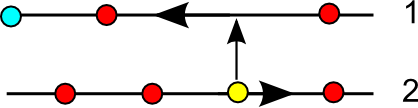
\includegraphics[width=.5\textwidth]{generatorexample.png}
\caption{\textbf{A PDMP on two species.} In this case $K^{(1)} = 1$, with $R^{(1)}_{21}= 1$. }  \label{genex}     
\end{centering}
\end{figure}

To allow for functionals which track empirical measures on $L_k$, in Section \ref{extension} we will construct an extended PDMP $\tilde X(t)$ from $X(t)$ with added dimensions that track boundary events. We can then select  functionals $F^\phi_k(\tilde {\textbf x})$ in the domain   $\mathcal D(\tilde {\mathcal A})$ of the extended generator $\tilde{\mathcal A}$.  These functionals satisfy condition (3) by adding a correction term to $f^\phi_k(\textbf{x})$, dependent on the extra dimensions in $\tilde{\textbf{x}}$.

For each species $k$, we will use $F^\phi_k(\tilde {\textbf x})$ to construct the martingales from (\ref{martingale}). These martingales involve empirical pairings  $\langle \mu^N,\phi\rangle$ and terms $B_{i,j}^{\phi,N}(t)$, which roughly describe total occurrences of boundary events.   We show the limit of these equations approaches (\ref{limeq}) as $N \rightarrow \infty$.  To do so, we first  show the martingale term $M_\phi^{k,N}(t)$ converges to zero in the local uniform metric, a consequence of Doob's theorem. The most technical part  involves the tightness of empirical pairings .  As in Chapter 2, we will use the Theorems \ref{Ald} and \ref{Cap} to show tightness of $\mu_k$.
 
Finally, we focus our attention on the terms $B_{i,j}^{\phi,N}(t)$. Using a law of large numbers type argument, we will show these  terms  converge in the local uniform metric to terms involving $\langle \mu_k, \phi\rangle$ and $F_k(t)$. 











\section{The extended PDMP $\tilde X^{N}(t)$}\label{extension}


 To address condition (3) of Theorem \ref{fourcond}, let us denote $\tau_i^{j,k}$ as the $i^{th}$ time that a boundary event reassigns a particle from $L_j$ to $L_k$. Note that $\tau_i^{j,k}$ may equal $\tau_m^{j,k}$ when $m>i$, since boundary events can reassign more than one particle.  Ordering of $\tau_i^{j,k}$  when several particles are simultaneously reassigned from $L_j$ to $L_k$  is done with respect to the same ordering used to determine reassignments $R_{jk}^{(l)}$.   Suppose we have $\kappa_{j,k}^N(t)$ particles $(x_1, \dots, x_{\kappa_{j,k}^N(t)})$ that have been reassigned from $L_j$ to $L_k$, at times  $\tau_i^{j,k}$. We now define \textbf{boundary variables} that track jumps from boundary events as 
\begin{equation}
B_{j,k}^{\phi,N}(t) = \sum_{i = 1}^{\kappa_{j,k}^N(t)} \frac{\phi(x_i)}{N} \quad \phi \in \mathcal C.
\end{equation}
  

 
We now define the extended PDMP $\tilde X^{N}(t)$ which tracks jumps occurring in $X^{N}(t)$.   Formally, we can write the extended state space as 
\begin{equation}
\tilde E = \coprod_{\vec s \in K } (\mathbb{R}^{|\mathbf s|+M^2}_+)_\mathbf s = \left\{(\mathbf s,\tilde{\mathbf x}):\mathbf s \in K, \tilde{\mathbf x} \in \mathbb{R}_+^{|\mathbf s| + M^2}\right\}. 
\end{equation}
A state $\tilde {\textbf{x}} \in \tilde E$ can be written as 
\begin{equation}
\tilde {\textbf{x}} = \left(x_1, \dots, x_{|\mathbf s|},b_{1}^1, \dots b_1^M, \dots, b_{M_-}^1, \dots, b_{M_-}^M\right).
\end{equation} 
The quantities $b_i^j$ are a means of recording the number and type of boundary events which occur.  We impose that boundary variables have no drift in $\tilde E$, which means that for vector fields in $\tilde{ \mathcal X}$, we let $\tilde{\mathcal X}_{\vec s}= \mathcal X_{\vec s}$, and define the exit boundary as
\begin{equation}
\tilde \Gamma^*(\tilde {\textbf{x}}) = \left\{(y, b_1^1, \dots, b_{M_-}^M)| y \in \Gamma^*\right \}.
\end{equation}
The main difference between $\tilde{\textbf{x}}$ and $\textbf{x}$ is seen in the extended transition kernel $\tilde Q$. For $\tilde {\textbf{x}}\in \tilde E$, the set of possible states  $\tilde E_{int}(\tilde {\textbf{x}})$ that $\tilde {\textbf{x}}$ may jump to from interior events is simply the the set $E_{int}(\textbf{x})$ with added unchanged boundary variables:
\begin{equation}
\tilde E_{int}(\tilde {\textbf{x}})  = \left\{(y, b_1^1,\dots, b_{M_-}^M)| y \in E_{int}(\textbf{x})\right\}.
\end{equation}
For $\tilde {\textbf{x}} \in \tilde \Gamma^*(\tilde E)$, however, boundary variables will increase, corresponding to the types of boundary events that occur at $\tilde{\mathbf x}$. Suppose a boundary event, triggered from a particle hitting the origin of $L_l$, selects particles $x_1, \dots, x_{K^{(l)}}$. We then define the new possible states of $\tilde {\textbf{x}}$ as 
\begin{equation}
\tilde E_b(\tilde {\textbf{x}})  = \left\{(y, \tilde b_1^1,\dots,\tilde  b_{M_-}^M)| y \in E_b(\textbf{x})\right\},
\end{equation}
where boundary variables change as 
\begin{equation}
\tilde b_i^j =  b_i^j+ \sum_{x_k\in L_i}\sum_{j = 1}^M \frac{\phi (x_k)}{N}\textbf{1}_{R^{(l)}_{ik} =j}, \quad i,j = 1, \dots, M . \end{equation}
Thus, boundary variables add the sum of quantities $\phi(x_k)$ to $b_i^j$, where $x_k$ is reassigned from $L_i$ to $L_j$.
We can then express the extended transition probability as  
\begin{equation}
\tilde Q(y,\tilde {\textbf{x}}) = \begin{cases}p_{b}(y,\tilde {\textbf{x}}) & \tilde {\textbf{x}} \in \tilde \Gamma^*, y\in \tilde E_b(\textbf{x}) \\
p_{i}(y,\tilde {\textbf{x}}) & \tilde {\textbf{x}} \in E, y \in \tilde E_{int}(\textbf{x})   \\
0 & otherwise. 
\end{cases}
\end{equation}
We thus have a well defined PDMP $\tilde X(t)$ determined from $\tilde E, \tilde{\mathcal X},$ and $ \tilde Q$. From here it is not hard to see that 
\begin{equation}
\tilde X(t) = \left(x_1(t), \dots, x_{|\mathbf s|}(t),B_{1,1}^{\phi,N}(t), \dots B_{1,M}^{\phi,N}(t), \dots, B_{M_-,1}^{\phi, N}(t), \dots, B_{M_-,M}^{\phi,N}(t)\right)
\end{equation} 


With the parameters $B_{j,k}^{\phi,N}(t)$ at our disposal, we may now define functionals
\begin{equation}
F^{\phi,N}_k(\tilde X(t)) = \sum_{x(t)\in L_k} \frac{\phi(x(t))}{N}+\sum_{j= 1}^M B_{j,k}^{\phi,N}(t)-B_{k,j}^{\phi,N}(t) , \quad k = 1, \dots, M. 
\end{equation}
\section{Reassignment bounds and martingale equations}
To show that  $F^{\phi,N}_k$ is a valid functional in the domain of the infinitesimal generator $\tilde{\mathcal{A}}$, we give a simple bound for jumps which will be utilized throughout this paper.  Denote the maximum number of reassigned particles at a critical event by 
\begin{equation}
K = K^{int} \vee \max_i K^{(i)}.
\end{equation}


\begin{lem}\label{jumpbound}  The number of particle interior events $m_{int}^N$ and  reassignments $\kappa^N(t)$ has bounds
\begin{enumerate}
\item (\textbf{Expectation for fixed} $N$) For any $N \in \mathbb N$, we have 
\begin{equation}
\mathbb{E} [m^N_{int}(t)]\le \beta Nt,
\end{equation}  and
\begin{equation}
\mathbb{E} [\kappa^N(t)]\le KN(1+\beta t).
\end{equation}

\item 
(\textbf{Law of large numbers bound})  
\begin{equation}
\limsup_{N\rightarrow \infty} \frac{m^N_{int}(t)}{N}\le \beta t    \quad a.s., 
\end{equation} 
and
\begin{equation}
\limsup_{N\rightarrow \infty} \frac{\kappa^N(t)}{N}\le K(1+\beta t)    \quad a.s.. 
\end{equation}


\end{enumerate}  
\end{lem}
\begin{proof} Clearly, the number of boundary events is bounded by the initial number of particles $N$.   The expected rate of interior events $m_{int}^N(t)$ can be bounded by the Poisson parameter $\beta(X^N(t)) = \beta (N(t))\le \beta N$.    The expected number of jumps up to time $t$ is thus bounded by $\beta Nt$, which proves (1).  

For part (2), we note that a Poisson process $P_\gamma(t)$ of intensity $\gamma$ at time $t$ satisfies the scaling argument
\begin{equation}
P_\gamma(t) \sim P_{a\gamma}(t/a) \quad a>0.
\end{equation}
It then follows  from the law of large numbers for Poisson processes,
\begin{equation}
\frac{P_\gamma(t)}{t} \rightarrow \gamma \quad a.s. \hbox{ as } t \rightarrow \infty,
\end{equation}
 that we can obtain  
\begin{eqnarray} 
\mathbb P(\limsup_{N \rightarrow \infty}\frac{m_{int}^N(t)}{N}>\beta t) \le \mathbb{P}\left(\limsup_{N \rightarrow \infty}\frac{P_{N\beta}(t)}{N} >\beta t\right)\\
= \mathbb{P}\left(\limsup_{N \rightarrow \infty}\frac{P_{\beta}(Nt)}{Nt}t > \beta t\right) = 0, \nonumber \end{eqnarray}    
which proves part (2).   
\end{proof}

\begin{theorem}\label{gencalcs}
For the domain of the infinitesimal generator $\mathcal D(\tilde {\mathcal A})$ corresponding to $\tilde x$, we have $F^{\phi,N}_k \in \mathcal D(\tilde {\mathcal A})$, for $k = 1,\dots, M$. 
\end{theorem}

\begin{proof} We need to show the four conditions of Theorem \ref{fourcond} hold for $F^{\phi,N}_k$.  Conditions (1) and (2) are clear, since particles in $\tilde E$ transport along a continuous flow, and $\phi \in C^1(\mathbb{R}^+)$.

For condition (4), we need to make estimates on the frequency of jumps in $\tilde E$.  We first note 

\begin{equation}
\mathbb E\left[B_{j,k}^{\phi,N}(t)\right] \le \mathbb E[\kappa^N(t)]\frac{\|\phi\|_\infty}{N}.  
\end{equation}
Let us define the the $m^N(t)$ jump times before time $t$ as $\tau_1, \dots, \tau_{m^N(t)}$. Then from Lemma \ref{jumpbound},
\begin{eqnarray}
\mathbb{E}\left[\sum_{i = 1}^{m^N(t)} |F_k^{\phi,N}(\tilde X(
\tau_i)-F_k^{\phi,N}(\tilde X(\tau_{i-1}))|\right]  \\
\le \mathbb{E}\Big [\sum_{i = 1}^{m^N(t)}|\langle \mu^N_k(\tau_i),\phi\rangle-\langle \mu^N_k(\tau_{i-1}),\phi\rangle|\nonumber\\+\sum_{j = 1}^M|B_{j,k}^{\phi,N}(\tau_i)-B_{k,j}^{\phi,N}(\tau_i)+ B_{j,k}^{\phi,N}(\tau_{i-1})-B_{k,j}^{\phi,N}(\tau_{i-1})|  \Big]\nonumber  \\
\le \frac{4M}N\mathbb{E}[\kappa^N(t)]\le\frac{4MK}N(\beta tN+N) \nonumber \\
< \infty.  \nonumber
\end{eqnarray}
The nontrivial part to show is the boundary condition (3).
 Note that for $X(\tau^-) \in \Gamma^*$, 
  \begin{eqnarray}
 \int_E F_k^{\phi,N}(y)-F(X(t^-)) Q(dy,X(t^-)) = \mathbb E(\Delta F_k^{\phi,N}(X(t)))\\
 =\mathbb E\left[\Delta \langle \mu_k^N(t), \phi \rangle \right]+\sum_j\mathbb E\left[\Delta B_{j,k}^{\phi,N}(t) -\Delta B_{k,j}^{\phi,N}(t) \right].\nonumber 
\end{eqnarray}
Assume that a  boundary event at jumping time $\tau$ occurs from a particle hitting the origin in $L_l$, and randomly selects $K^{(l)}$ particles $(x_1, \dots, x_{K^{(l)}})$.  Then we have the expected change in empirical measure as a sum of the averages resulting from particles leaving and entering $L_k$: 
\begin{align}  
&\mathbb E[\Delta \langle \mu_k^N(\tau, \phi) \rangle ] = K^{(l)}p_k^{(l)}(\tau)\cdot\mathbb{E}\left[\frac{\phi(x_1)}{N}|x_1 \in L_k \right]\\&+\sum_{i= 1}^{M}\sum_{ j = 1}^{K^{(l)}}p_i^{(l)}(\tau) \cdot\mathbb{E}\left[\frac{\phi(x_1)}{N}|x_1 \in L_i \right]\mathbf{1}_{R^{(l)}_{ij} = k}\nonumber\\
&=  - \frac{K^{(l)}w^{(l)}_k}{N^{l}} \langle \mu_k^N(\tau), \phi \rangle +\sum_{i= 1}^{M}\sum_{ j = 1}^{K^{(l)}} w^{(l)}_i\frac{\langle \mu_i^N(\tau), \phi \rangle}{N^{(l)}}\mathbf{1}_{R^{(l)}_{ij} = k}. \nonumber 
\end{align}
However, we see that for jumps in the boundary variables,
by similar calculations, at a boundary jumping time $\tau$ 
\begin{equation}
\sum_j\mathbb E\left[\Delta B_{j,k}^{\phi,N}(\tau)\right] = \sum_{i = 1}^{M} \sum_{m= 1}^{K^{(l)}} w^{(l)}_i\frac{\langle \mu_i^N(\tau), \phi \rangle}{N^{(l)}}\mathbf{1}_{R^{(l)}_{im} = k}
\end{equation}
for expectations of particles entering species $k$, and   
\begin{align}
\sum_j\mathbb E\left[\Delta B_{k,j}^{\phi,N}(\tau)\right]  &=  -K^{(l)}p_k^{(l)}(\tau)\mathbb{E}\left[\frac{\phi(x_1)}{N}|x_1 \in L_k\right] \\ 
&= \frac{K^{(l)}w^{(l)}_k}{N_{l}} \langle \mu_k^N(\tau), \phi \rangle \nonumber  \end{align}
for particles leaving species $k$.
\end{proof}
  In the following, define the empirical total number as
  \begin{equation}
  G^N(s)=\sum_{k = 1}^M \langle \mu_k^N(\tau), 1 \rangle, \quad G^{int,N}(s)=\sum_{k = 1}^M w_k^{int}\langle \mu_k^N(\tau), 1 \rangle 
  \end{equation}
  To each $F_k^{\phi,N}$, we can now construct the following martingale.  

\begin{theorem} For $k \in \{1, \dots, M\}$, the quantity 
\begin{align}\label{mgaleeqn}
&M_k^{\phi,N}(t) = \langle \mu_k^N(t), \phi\rangle- \langle \mu_k^N(0), \phi\rangle+\\
&\sum_{j= 1}^M B_{j,k}^{\phi,N}(t)-B_{k,j}^{\phi,N}(t) -\int_0^t \langle \mu_k^N(s), \phi' v_k \rangle +\nonumber \\
&\frac{\beta G^N(s)}{G^{int,N}(s)} \left[K^{int}w^{int}_k \langle \mu_k^N(s),\phi\rangle\frac{}{}-\sum_{i = 1}^{M}\sum_{j = 1}^{K^{int}}\  w^{int}_i \langle \mu_i^N(s),\phi\rangle\mathbf{1}_{R^{(l)}_{ij} = k}\right]ds \nonumber  
\end{align}
is a martingale.
\end{theorem}

\begin{proof}
The vector field $\tilde{\mathcal X}$ acts only on the first $N$ coordinates of $\tilde x$, and satisfies
\begin{eqnarray}
 \tilde{\mathcal X}(F_k^{\phi,N}(\tilde x)) = \sum_{i = 1}^{N} \sum_{x_i \in L_k}v_{s_i}(x_i)\frac{\partial}{\partial x_i}\frac{\phi(x_i)}{N} = \sum_{x_i \in L_k} v_k(x_i)\frac{\phi'(x_i)}{N} \\
 = \langle \mu_k^N, \phi' v_k \rangle \nonumber 
 \end{eqnarray}
Using equation (\ref{generator}), our formula for the extended generator is then
\begin{align}\label{genequa}
\tilde{\mathcal A}(F_k^{\phi, N}(\tilde x))&  \\ &=\langle \mu_k^N, \phi' v_k \rangle -\beta(\tilde x)\int_E (F_k^{\phi, N}(y)-F_k^{\phi, N }(\tilde x))Q(dy;\tilde x)) \nonumber\\
&= \langle \mu_k^N, \phi' v_k \rangle -\beta N \mathbb{E}\left[\Delta(F_k^{\phi, N}(\tilde x))\right].\nonumber 
\end{align}  
The calculation of the change of the functional over interior events is similar to Theorem \ref{gencalcs}:
\begin{align}\label{intfunct}
 &\mathbb{E}\left(\Delta(F_k^{\phi, N}(\tilde x))\right)=  \frac{K^{int}p^{int}_k }{|L_{k}|} \langle\mu_k^N,\phi\rangle-\sum_{i = 1}^{M}\sum_{j=1}^{K^{int}}  \frac{p^{int}_i }{|L_{i}|}\langle \mu_i^N,\phi\rangle\mathbf{1}_{R^{(l)}_{ij} = k}\\ 
&= \frac{1}{G^{int,N}(s)}\left[K^{int}w^{int}_k \langle \mu_k^N(s),\phi\rangle\frac{}{}-\sum_{i = 1}^{M}\sum_{j = 1}^{K^{int}}\  w^{int}_i \langle \mu_i^N(s),\phi\rangle\mathbf{1}_{R^{(l)}_{ij} = k}\right]. \nonumber 
\end{align}

Combining terms, we see the martingale $M_k^{\phi,N}(t)$ defined from equation (\ref{martingale}) then coincides with (\ref{mgaleeqn}).  
\end{proof}

We now uniformly bound the martingale $M^{\phi,N}_k(t)$, which will decay to zero in the mean $L^\infty$ metric.  
\begin{theorem} For $t<T_e$ we have 
\begin{equation}
\mathbb{E}[\sup_{s \in [0,t]}(M_k^{\phi,N}(s))] \le \frac{(4M+2)K\|\phi\|_\infty\sqrt{1+\beta t}}{\sqrt N},
\end{equation}
\end{theorem}
\begin{proof}

We bound jumps in $M^{\phi,N}_k(t)$ by noting that at most $K$ particles are either reassigned in a critical event: 

\begin{equation}
|\Delta M_k^{\phi,N}(t) |= |\Delta\langle \mu^{N}_k(t),\phi\rangle|+|\Delta (\sum_{j = 1}^M B_{j,k}^{\phi,N}(t)+B_{k,j}^{\phi,N}(t))|\ \le \frac{(2M+1)K\|\phi\|_\infty}N. \end{equation}

It then follows that, from Lemma \ref{jumpbound}, that
\begin{align}\label{martinq}
&\mathbb E[M_k^{\phi,N}(t)^2] = \mathbb{E}\left [\sum_{i = 1}^{m_N(t)}\Delta M_k^{\phi,N}(\tau_i)^2\right ]\\
&\le\frac{(2M+1)^2K^2\|\phi\|^2_\infty}{N^2} \mathbb{E}[m_N(t)]\le \frac{(2M+1)^2K^2\|\phi\|^2_\infty(1+\beta t)}{N}. \nonumber   
\end{align}

 

We now use Doob's inequality to obtain
\begin{equation}\label{moarmartinq}
\mathbb{E}\left[\sup_{s \le t}|M_k^{\phi,N}(s)|\right]^2 \le \mathbb E\left[\sup_{s \le t} M_k^{\phi,N}(s)^2\right] \le 4\mathbb E[M_k^{\phi,N}(t)^2].
\end{equation}
The result follows from applying (\ref{martinq}) to (\ref{moarmartinq}).
\end{proof}

\section{Existence of limiting measures}\label{cogito}

We base the existence interval $T_e>0$ off of when species will have positive total numbers almost surely.  The following lemma ensures that the transition probabilities, and subsequently the kinetic equations (\ref{limeq}), are well defined. The technical details of the the following lemma will be utilized in Lemma \ref{geometric} in determining tightness of empirical measures. The existence time $T_e$ will eventually be extended to a reasonable time where the solution is well defined as long as each species has positive total particle number.    



\begin{lem}\label{mintime} There exists a time $T_e$ where, for all $k = 1, \dots, M$, and $0<t<T_e$, the following hold: \begin{enumerate}
\item (\textbf{Fraction loss of particles})  
\begin{equation}
\limsup_{N \rightarrow \infty} \sup_{0\le s\le t}g_k^N(s)>\frac 23g_k^0  \quad \hbox{ a.s.. }
\end{equation}
\item (\textbf{Total number of particles lost}) The quantity $H^{N}(t)=1-\sum_k g_k^N(t)$ is bounded by a fraction of the total number in each species:
\begin{equation}
\limsup_{N \rightarrow \infty}H^N(t)<\frac 1{3M^2K}\mu_k^0(\mathbb{R}^+) \quad \hbox{ for all } k \in \{1, \dots, M\} \quad \hbox{a.s..}
\end{equation}
\item
(\textbf{Fixed time bound}) The time $T_e$ is bounded by a constant determined from fixed parameters in $X$
\begin{equation}
T_e < \frac{\min_k g_k^0}{4\beta M^2K}.
\end{equation}
\end{enumerate}


\end{lem}

\begin{proof}
Denote the flow determined from vector fields $v_i$ at time $t$ on $L_i$ as $\varphi^i(t,x)$, with initial condition $\varphi^i(0,x) = x$. Regardless of the choice of reassignment of particles, the total particle number lost  from boundary deletions $H^{N}(t)$ can be crudely bounded by
\begin{equation}
\limsup_{N\rightarrow \infty} \sup_{0\le s\le t}H^N(s) \le \sum_{i = 1}^M \mu_k^0([0,a(t)]), 
\end{equation}
for all $N<\infty$, where $\varphi^i(s,a(t))>0$ for all $s\le t$ in $L_i$.  
Since the initial measures $\mu_k$ are nonatomic, we can choose $t_1$ such that
\begin{equation}\label{massbound}
\sum_{k = 1}^M \mu_k^0([0,a(t_1)])<\min_{1\le i \le M} \frac 1{3M^2 K}g_i^0  ,
\end{equation}
which shows part (2).  

We now show  part (1).  As noted in Lemma \ref{jumpbound}, the rate of interior events is bounded by $\beta N$, which means that the total particle total number lost through interior events $H_{int}^N(t)$ has the bound 
\begin{eqnarray}
\limsup_{N\rightarrow \infty}H_{int}^N(t_2^1) \le K\beta t_2^1\\<\min_{1\le i \le M} \frac 1{6}g_i^0 \quad a.s. \nonumber
\end{eqnarray}
for a sufficiently small $t_2^1>0$. Total loss from boundary events $H_{b}^N(t)$ satisfies the bound
\begin{eqnarray}
\limsup_{N\rightarrow \infty}H_{b}^N(t_2^2) \le\sum_{k = 1}^M \mu_k^0([0,a(t_2^{2})])\\<\min_{1\le i \le M} \frac 1{6}g_i^0, \nonumber
\end{eqnarray}  
for a sufficiently small $t_2^2>0$.  Letting $t_2 = t_2^1 \wedge t_2^2$ then shows part (1), and letting 
  
\begin{equation}
T_{e}=t_1\wedge t_2 \wedge \frac{1}{2\beta MK} 
\end{equation}
gives a positive time $T_e>0$ that satisfies all three conditions.
\end{proof}

In the following, denote the set of intervals $I_\delta$ of  length at most $\delta$ as
\begin{equation}
I_\delta = \{(a,b)\subset \mathbb{R}^+, b-a<\delta\}.
\end{equation}


Our method of proof shows  that the sequences $\mu_k^N(t)$ are approximately nonatomic with probability one as $N\rightarrow \infty$. We make this rigourous with the following definition.
\begin{deef}
 A sequence of random measure processes $\nu_t^n$ is \textbf{probabilistically approximately nonatomic} (p.a.n.a.) for time $T$ if for all $\eta > 0$,  \begin{equation}\label{paac}
 \lim_{\delta \rightarrow 0}\sup_{I \in I_\delta}\limsup_{n\rightarrow \infty} \sup_{t \in [0,T]}\mathbb P(\nu_t^n(I) >\eta) = 0 .
\end{equation}
\end{deef}
We will eventually demonstrate that the p.a.n.a. property is sufficient to show the Aldous conditions of Theorem \ref{Ald}. We aim to  express $\mu_k^N(t)$ by a decomposition of particles though their histories as different species. With this in mind, we have the following definition, which isolates subsets of particles in species $k$.

\begin{deef} A finite measure process $\mathscr A_k^N(t) \in \mathcal M(\mathbb{R}^+)\times [0,T_e]$   is a  \textbf{subparticle measure process of}  $\mu_k^N(t)$ if \begin{equation}
\mathscr A_{k}^N(t)= \sum_{\substack{x \in S^N(t) \\ }} \frac{\delta_{x}}{N}.
\end{equation}
for some support $S^{N}(t) \subset L_k$ satisfying $S^{N}(t) \subset S_k(X^{N}(t))$. \end{deef}



Given a subparticle measure process $\mathscr A_{j}^N(t)$ with support $S^{N}(t)$ , we can then define empirical measures of particles in $S^N(t)$ that jump from $L_j$ to $L_k$ and then flow on $v_k$ with no probability of jumping again. 


\begin{deef}
A \textbf{boundary running measure} $ \tilde{\mathscr A}_{j,k}^N(t) \in \mathcal M(\mathbb{R}^+)\times [0,T_e]$ of a subparticle measure process $\mathscr A_{j}^N(t)$ with support $S^{N}(t)$ is a measure of the form
\begin{equation}
\tilde{\mathscr A}_{j,k}^N(t) = \sum_{x\in U^k(s)}  \frac{\delta_{\varphi^k(\varphi^j(s, x), t-s)}}{N}
\end{equation}  
 with support
\begin{equation}
U^k(\tau) = \{x\in S^N(\tau^-) | \hbox{A boundary event at $\tau$ transfers $x$ to $L_k$}\}.
\end{equation}


We will denote the jump times of a running measure as $\tilde \tau_1,\dots, \tilde \tau_{\tilde m(t)}$, and the particles selected as $\tilde x_1, \dots, \tilde x_{\tilde m(t)}$, where $\tilde m(t)$ is the total number of such jumps.
\end{deef}
We can similarly define \textbf{interior running measures} $\tilde{\mathscr A}_{j,k}^{int,N}(t)$ for particles that jump from $L_j$ to $L_k$ due to interior events.  

\begin{theorem}\label{pacthm}  For $j,k = 1, \dots, M$ and  $t\in [0,T_e]$,  if the sequence of subparticle measure processes $R_j^N(t)$ is p.a.n.a., then so are running measures $\tilde R_{j,k}^{int,N}(t)$ and $\tilde R_{j,k}^{N}(t)$.
\end{theorem}

\begin{proof} 
Let $t \le T_e$.  
 Suppose a particle is chosen to transfer from $L_j$ to $L_k$ at time $s\le t$.  At a boundary event, after choosing a species $L_j$, particles are chosen uniformly on $L_j$ to reassign to another species. Thus, the (random) probability $q^N_s(I)$ of reassignment of a particle in the support of $R_j^N(s)$ in the correct interval at time $s$ before traveling to $I$ satisfies
\begin{equation}
q_s^N(I) = \frac{R_j^N(s)( \varphi^k(I, s-t))}{g_k^N(s)}.
\end{equation}
By the p.a.n.a. property of $R_j^N(t)$, for $\varepsilon>0$, there exists $\delta>0$ where for all $I \in I_\delta$
\begin{align}\label{probrightspec}
&\limsup_{N\rightarrow \infty} \sup_{s\le t} \mathbb P(q^N_s(I)>\varepsilon)\\
&\le \limsup_{N\rightarrow \infty} \sup_{s\le t}\mathbb P(R_j^N(s)( \varphi^k(I, s-t))> \frac{2g^0_k}{3}\varepsilon)<\varepsilon\nonumber
\end{align}
  The factor $2g_k^0/3$ arises from part 2 of Lemma \ref{mintime} , which bounds the total number of a particular species.
We now note that, from Markov's inequality, and part  2 of Lemma \ref{jumpbound}, for $I \in I_\delta$, 
 \begin{align}
 &\limsup_{N\rightarrow \infty} \sup_{t \in [0,T_e]}\mathbb P(\tilde R_{k,j}^{N}(t)(I) >\eta)\\
 &\limsup_{N\rightarrow \infty} \sup_{s \in [0,t]} \frac{\mathbb E\left[\tilde R_{j,k}^{N}(t)(I)\right]}{\eta}\le  \frac{K(1+\beta t)}{\eta}\limsup_{N \rightarrow \infty} \sup_{s\le t}\mathbb{E}(q_s^N(I)) \nonumber\\
 \nonumber \\  &\frac{K(1+\beta t)}{\eta}\limsup_{N \rightarrow \infty} \sup_{s\le t} \Big[\mathbb{E}(q_s^N(I)|q_s^N(I)>\varepsilon))\mathbb P(q_s^N(I)>\varepsilon)\nonumber\\&+\mathbb{E}(q_s^N(I)|q_s^N(I)>\varepsilon))\mathbb P(q_s^N(I)>\varepsilon)\Big]\nonumber\\&\le  \frac{K(1+\beta t)}{\eta} 2\varepsilon  \nonumber, 
\end{align}
As $\varepsilon$ is arbitrary, we may take $\delta\rightarrow 0$ to obtain our result. For interior particle submeasures, the proof is identical.   
\end{proof}

With probability one, a particle starting in $L_i$ at time $0$  visits a finite set of species  before arriving at its final destination at time $t$.  Suppose a particle $x(t)$ at time $\tau_k$ jumps from $L_{\sigma_k}$ to $L_{\sigma_{k+1}}$, for $k = 1, \dots, m$.  The locations of $x(t)$ can then be symbolically described through the following \textbf{path notation} $\mathcal P (x(t)) = (\Sigma(x(t)), \Theta(x(t)))$, with path location $\Sigma(x(t)) \in \{1, \dots , M\}^m, $ and jump description $\Theta(x(t)) \in \{\partial, I\}^{m-1}$.  Specifically, if $\Sigma(x(t))_i = \sigma_i$, and $\Sigma(x(t))_{i+1} = \sigma_{i+1}$, then $x(t)$ jumps from $L_{\sigma_i}$ to $L_{\sigma_{i+1}}$ at the $i^{th}$ jump time $\tau_{i}$. If $\Theta(x(t))_i = \partial$, then the $i^th$ jump is a boundary event at $\tau_i$, while $\Theta(x(t))_i = I$, denotes an interior event. The number of different species realized by a particle, or the length of a path, will be denoted $| \Sigma(x(t))|$.

We now define  \textbf{path measures} that keep track of particles that follow specific paths. for $\Sigma \in \{1, \dots , M\}^m$, denote
\begin{equation}
R_{\Sigma}(t)  = \{x(t) \in S_{\sigma_{|\Sigma|}}(t)|\Sigma (x(t)) = \Sigma \},
\end{equation}
and
\begin{equation}
\mu^N_{\Sigma}(t)= \sum_{x\in R_\Sigma(t)} \frac{\delta_x}{N}.
\end{equation}
It's straightforward to see that  $\mu^N_\Sigma(t)$ are subparticle measures. Path measures $\mu^N_\Sigma(t)$ with support $R_{\Sigma}(t)$ also have the following \textbf{no return property}: Suppose we track a specific particle $x(s) \in E$, with initial position $x_0 \in E$. If $x(t) \in R_{\Sigma}(t)$, and there exists $t'>t$ with $x(s) \in R_{\Sigma}(t')$, then $x(s) \in R_{\Sigma}(s)$ for $s \in [t,t']$. 

 The no return property ensures that a particle that is a member of $R_{\Sigma}(t)$ is not permitted to exit and reenter $L_k$. The importance of such a property will become apparent in the following theorem.  Denote the running measures of  $\mu^N_\Sigma(t)$ from $L_{\sigma_{|\Sigma|}}$ to $L_k$ as $\tilde \mu^N_{\Sigma,k}(t)$ and $\tilde \mu^{\beta,N}_{\Sigma,k}(t)$. We then have the following

\begin{theorem} \label{paacproof}
 $\mu^N_\Sigma(t), \tilde \mu^N_{\Sigma,k}(t)$,and $\tilde \mu^{\beta,N}_{\Sigma,k}(t)$ are p.a.n.a. for length $T_e$.
\end{theorem}

\begin{proof}We prove the theorem by induction on the path length $|\Sigma|$ .  For the base case,   $|\Sigma|= 1$ corresponds to particles which have not yet jumped from their initial distribution.  Thus the support of $\mu_\Sigma^N(t)$ is strictly contained in the support of the pullback measure $(\varphi^{\sigma_1})^*\mu^N(t)$, and is thus p.a.n.a., which implies that, from Theorem \ref{pacthm}, $\tilde \mu^N_{\Sigma,k}(t)$ and $\tilde \mu^{\beta,N}_{\Sigma,k}(t)$ are also p.a.n.a..

For the inductive step, suppose that for $|\Sigma|\le n$, $\mu^N_\Sigma(t), \tilde \mu^N_{\Sigma,k}(t)$, and $\tilde \mu^{\beta,N}_{\Sigma,k}(t)$ are p.a.n.a.. 
 For $k = 1, \dots, M$, let  $\tilde\Sigma = \Sigma *k$, where $|\Sigma|= n$ and $*$ denotes concatenation. Then $\mu^N_\Sigma$ is p.a.n.a., since the support of $\tilde \mu^N_{\Sigma,k}(t)$  contains the support of  $\mu_{\tilde \Sigma}^N(t)$, which follows from the no return property. This proves the induction step for $\mu^N_\Sigma(t)$.  Then we again have from  Theorem \ref{pacthm} that for $j =  1, \dots, M$, $\tilde \mu^N_{\tilde \Sigma,k}(t)$ and $\tilde \mu^{\beta,N}_{\tilde \Sigma,k}(t)$ are p.a.n.a., since $\mu^N_{\tilde \Sigma}(t)$ are subparticle measures. This completes the inductive step, and our result follows.    
\end{proof}

We need one more lemma to show that our empirical measures are p.a.n.a., namely that total numbers of empirical measures decrease subgeometrically with respect to  the length of paths.

\begin{lem}\label{geometric} For $t< T_e$,   $ \limsup_{N\rightarrow \infty} \mu_{ \Sigma}^N(t)(\mathbb{R}^+)\le c^{|\Sigma|}$ a.s., where  $c<\frac3{4M}$.
\end{lem}

\begin{proof}If suffices to show that both $\limsup_{N\rightarrow \infty}  \tilde \mu^N_{ \Sigma,k}(t)(\mathbb{R}^+) \le \limsup c\mu_{ \Sigma}^N(t)(\mathbb{R}^+)$ and  $\limsup \tilde \mu^{\beta,N}_{ \Sigma,k}(t)(\mathbb{R}^+) \le \limsup c\mu_{ \Sigma}^N(t)(\mathbb{R}^+)$ a.s.. We'll first show the inequality for boundary running measures.  Recall from Lemma \ref{mintime}, that for $t<T_e$, we can ensure that 
\begin{enumerate}
\item $\limsup_{N\rightarrow \infty} g_k^N(s)> \frac{2}{3} g_k^0$, and 
\item
$\limsup_{N\rightarrow \infty} H^{N}(t)< \frac{1}{3 M^2K}g_k^0$,
\end{enumerate} 
 hold almost surely. Suppose first $\limsup_{N\rightarrow \infty} \mu_{ \Sigma}^N(t)(\mathbb{R}^+)\ge  \frac{g_k^0}{2M}$. Since the maximum total number of particles that can leave a species $L_k$ from boundary events is bounded by $K H(t)$,   Condition (2) of Lemma \ref{mintime} implies  for $k \in \{1, \dots, M\}$, 
\begin{equation}
\limsup_{N\rightarrow \infty} \tilde \mu^N_{ \Sigma,k}(t)(\mathbb{R}^+)\le  \frac{1}{3 M^2}g_k^0. 
\end{equation}

But by the assumption on $\mu_{ \Sigma}^N(t)(\mathbb{R}^+)$,
\begin{equation}
 \frac{1}{3 M^2}g_k^0 \le  \frac 2{3M}\limsup_{N\rightarrow \infty} \mu_\Sigma^N(s)(\mathbb{R}^+).
\end{equation}
     
On the other hand, if $\limsup_{N \rightarrow \infty} \mu_{ \Sigma}^N(t)(\mathbb{R}^+)\le  g_k^0/2M$, then we  know from condition (1) of Lemma \ref{mintime} that the probability of any particle chosen from $L_k$ being in the support of $\mu_\Sigma^N(s)$ has probability less than  $(g_{k}^{0}/2M)/(2g_k^0/3) = 3/(4M)$. Thus,
\begin{equation}
\limsup_{N\rightarrow \infty} \tilde \mu^N_{ \Sigma,k}(t)(\mathbb{R}^+) \le \frac 3{4M}\limsup_{N\rightarrow \infty} \mu_\Sigma^N(s)(\mathbb{R}^+)  \quad a.s.  
\end{equation}
To bound interior probabilities, we again use  Lemma \ref{mintime}, but now use condition (3), where $T_e$ satisfies $K \beta M^{2}T_e <\min_k g_k^0/4$.  Then, as the Poisson rate is bounded by $\beta N$, we have from Lemma \ref{jumpbound} that the total number of species reassignments is bounded by
\begin{equation}
\limsup_{N\rightarrow \infty}K\frac{m_{int}^N(t)}{N}\le K\beta t\le   \frac {\min_i g_i^0}{4M^2}  \quad a.s.
\end{equation}
  Thus, we can apply an argument similar to the case  of boundary events, where we again compare  $\limsup_{N \rightarrow \infty} \mu_{ \Sigma}^N(t)(\mathbb{R}^+)$ with $g_k^0/2M$ to obtain    
 \begin{equation}
 \limsup_{N\rightarrow \infty} \tilde \mu^{\beta,N}_{ \Sigma,k}(t)(\mathbb{R}^+) \le  \frac 3{4M}\limsup_{N\rightarrow \infty} \mu_\Sigma^N(t)(\mathbb{R}^+)         \quad a.s.
\end{equation}
\end{proof}

\begin{theorem} Let $t< T_e$. The empirical measures $\mu_k^N(t)$ are p.a.n.a.
\end{theorem}
\begin{proof}
Let $\eta>0$.  We can decompose $\mu_k^N(t)$ as
\begin{equation}
 \mu_k^N(t) = \sum_{(\Sigma, \Theta) \in \mathcal P} \mu_\Sigma^N(t) =\sum_{j = 1}^\infty \sum_{\substack{ |\Sigma | = j\\\sigma_{|\Sigma|} = k}} \mu_\Sigma^N(t).
\end{equation}

Let $\eta>0$, and choose $L$ so that $\mu^N_\Sigma(t)(\mathbb{R}^+) \le \eta/8$ for $|\Sigma|> L$ (This is possible through Lemma \ref{geometric}).   There are $M_L:=M\sum_{j = 1}^{L-2}(M-1)^{j-1}$ paths where $|\Sigma|\le L$ and $\sigma_{|\Sigma|} = k$  ($M$ initial paths and $M-1$ options for each new transition). From Lemma \ref{paacproof}, each of these path measures are  p.a.n.a., meaning that
  \begin{equation}\label{paaclower}
  \lim_{\delta \rightarrow 0}\lim_{I \in {I_\delta}}\limsup_{N\rightarrow \infty}\sup_{s \in [0,T_e]}\mathbb{P}(\mu_\Sigma^N(s)(I)>\tilde \eta) = 0 
  \end{equation}
  with 
\begin{equation}
\tilde \eta = \frac{\eta}{2M_L},
\end{equation}
 for any $\mu_\Sigma^N(t)$ with $|\Sigma|<L$. But then we have, for any $t \in [0, T_e]$,
and $I \in I_\delta$, 
\begin{align}
&\limsup_{N\rightarrow \infty}\sup_{t \in [0,T_e]}\mathbb{P}(\mu_k^N(t)(I)>\eta)\\
&= \limsup_{N\rightarrow \infty} \sup_{t \in [0,T_e]}\mathbb P \Big(\sum_{j = 1}^\infty \sum_{\substack{ |\Sigma | = j\\\sigma_{|\Sigma|} = k}}\mu_\Sigma^N(t)(I)>\eta\Big ) \nonumber \\
&\le \limsup_{N\rightarrow \infty}  \sup_{t \in [0,T_e]}\mathbb P\Big(\sum_{j = 1}^{L} \sum_{\substack{ |\Sigma | = j\\\sigma_{|\Sigma|} = k}} \mu_\Sigma^N(t)(I)  +\frac{\eta}8\sum_{j > L}\sum_{\substack{ |\Sigma | = j\\\sigma_{|\Sigma|} = k}} \mu_\Sigma^N(t)(\mathbb{R}^+)>\eta\Big)\nonumber \\
&\le \limsup_{N\rightarrow \infty}  \sup_{t \in [0,T_e]}\mathbb P\Big(\sum_{j = 1}^{L} \sum_{\substack{ |\Sigma | = j\\\sigma_{|\Sigma|} = k}} \mu_\Sigma^N(t)(I)  +\frac{\eta}8\sum_{j = 1}^\infty (cM)^j>\eta\Big)\nonumber \\
 &\le \limsup_{N\rightarrow \infty} \sup_{t \in [0,T_e]}\mathbb P\Big(\sum_{j = 1}^L \sum_{\substack{ |\Sigma | = j\\\sigma_{|\Sigma|} = k}} \mu_\Sigma^N(t)(I)  >\eta/2\Big)\nonumber \\
 &\le 1-\limsup_{N\rightarrow \infty}\sup_{t \in [0,T_e]}\mathbb  P( \mu_\Sigma^N(t)(I))  \le\tilde \eta) \hbox { for all } |\Sigma|<L.\nonumber 
\end{align}
By (\ref{paaclower}), this quantity approaches 0 as $\delta \rightarrow 0$.
\end{proof}
Here we show the Aldous conditions, which are a direct property of the p.a.n.a. property of $\mu^N_k(t)$.

\begin {lem}
The Aldous conditions of Lemma \ref{Ald} hold for $\mu^N_k(s)$
\end {lem}

\begin{proof} Condition (1) follows trivially, since we have for all $t \in [0, T_e]$,  
\begin{equation}
|\langle \mu_k^N,\phi \rangle|<\|\phi \|_\infty,
\end{equation}
meaning that (1) holds for $ L = \|\phi\|_\infty$.  For condition (2), we observe that particles from time $t$ to $t+s$ either drift on $L_k$, are deleted, or are reassigned to a new species. 
\begin{align}
&\limsup_{N\rightarrow \infty} |\langle\phi,\mu_k^N((\tau+s )\wedge T_{e})\rangle \  - \langle\phi,\mu_k^N(\tau)\rangle|  \\&= \limsup_{N\rightarrow \infty}\left| \int_{\mathbb{R}^+}\phi(x) (\mu_k^N((\tau+s) \wedge T_{e})- \mu_k^N(\tau))(dx)\right | \nonumber \\\label{firsteq}
&\le \limsup_{N\rightarrow \infty} \left | \int_s^\infty (\phi(\varphi^k (x,s))-\phi(x))\mu_k^N(\tau)(dx) \right | \nonumber \\
&+\|\phi\|_\infty (K+1)\left(\sum_{i = 1}^{M_-}\mu_{i}^N(\tau)([0,\varphi^i (0,-s)])+s\beta\right) \quad a.s. \nonumber 
\end{align}
The last inequality uses the fact, from  Lemma \ref{jumpbound} that almost surely at most a $s\beta$ total number are reassigned from interior events,   and that $(K+1)(\sum_{i = 1}^{M_-}\mu_{i}^N(\tau)([0,\varphi^i (0,-s)])$ particles will either be reassigned or deleted due to boundary events. 
We can use the continuity and boundedness of $\phi$ and $\varphi$ to estimate  (\ref{firsteq}).  For all $R>0$:
\begin{eqnarray}\label{infbound}
\left| \int_s^\infty (\phi(\varphi^k(x,s))-\phi(x))\mu_k^N(\tau)(dx) \right |\\
\le \|\phi(\varphi^k(x,s))-\phi(x)\|_{L^\infty([0,R])}+2\|\phi\|_\infty \mu_k^N(s)([R,\infty])\nonumber 
\end{eqnarray}
The first term tends to 0 as $s\rightarrow \infty$.  For the second term, we can always find $R$ large enough where only a small total number enters $[R, \infty]$ in any $L_k$.  Precisely, for all $\varepsilon$, there is an $R = R(\varepsilon)$ where 
\begin{eqnarray}
\sum_{i = 1}^M \mu_k^0([R,\infty))<\varepsilon/2, \quad  \sum_{i = 1}^M\mu_k^0([R/2, R]) < \varepsilon/2, \\
\varphi^k(R/2, t)<R, \quad t \in [0,T_e]. \nonumber 
\end{eqnarray}
 These bounds are thus independent of $N$ and $s$. Thus, since $R$ is arbitrary, (\ref{infbound}) tends to 0 as $s\rightarrow 0$.  For the second term of (\ref{infbound}) , notice that from the   p.a.n.a. property of $\mu_k^N(t)$,we have, for $\eta>0,$
\begin{equation}\label{absinq}
\lim_{s \rightarrow 0}\limsup_{N\rightarrow \infty}\sup_{\tau \in [0,T_e]}\mathbb P\left(\mu_k^N(t)([0,\varphi^k (0,-s)])>\frac{\eta}{MK\|\phi\|_\infty }\right) = 0.
\end{equation}

Thus we finally have, for any $\eta>0$,
\begin{align}
&\lim_{s\rightarrow 0}\limsup_{N\rightarrow \infty}\sup_{\tau \in [0,T_e]}\mathbb{P}(|\langle\phi,\mu_k^N(\tau+s \wedge T)\rangle \  - \langle\phi,\mu_k^N(\tau)\rangle|\ge\eta) \\
 &\le  \lim_{s\rightarrow 0}\limsup_{N\rightarrow \infty}\sup_{\tau \in [0,T_e]}\mathbb{P}\left(\|\phi\|_\infty K\sum_{i = 1}^M\mu_{k}^N(\tau)([0,\varphi^k (0,-s)])\ge\eta\right) \nonumber \end{align}
which approaches zero from (\ref{absinq}), meaning that Aldous' conditions are satisfied.
\end{proof}
By Lemma \ref{Cap}, we have shown tightness of random variables $\langle \mu_k^N(t), \phi\rangle$,   $\phi \in C_b(\mathbb{R}^+)$.  We can now use Lemma \ref{Ald} to obtain existence of a limiting measure,$\mu_k\in \mathcal{M}(\mathbb{R}^+)$ where for $\phi \in C_b(\mathbb{R}^+),$ there exists a subsequence $N_k$ with                  
\begin{equation}\label{pairbound}
\langle \phi, \mu_k^{N_k}(s) \rangle \rightarrow \langle \phi, \mu_k(s) \rangle
\end{equation}
in the local uniform topology for all $\phi \in C_b(\mathbb{R}^+).$  We now show the measures $\mu_k(s), k = 1,\dots, M$ are nonatomic almost surely.

\begin{theorem} Let  $k = 1, \dots, M$ and $t \in [0,T_e]$.
For any point $p \in \mathbb{R}^+$, the measures $\mu_k(t)$ satisfy
\begin{equation}
\mathbb P(\mu_k(t)(\{p\}) = 0) = 1. 
\end{equation}
\end{theorem}
\begin{proof}
Let $\eta>0$.  We will denote
\begin{equation}
I_\delta^p = \{I \in I_\delta | p \in I\}.
\end{equation}
Using the p.a.n.a. property, we have, for $\delta>0$, 
\begin{eqnarray}
\mathbb{P}(\mu_k(t)(\{p\}) > \eta)\le \limsup_{N\rightarrow \infty} \mathbb{P}(\mu_k(t)(\{p\})>\eta)\\
\le \sup_{I \in I_\delta^p}\limsup_{N\rightarrow \infty} \mathbb{P}(\mu_k(t)(I) > \eta)\rightarrow 0 \quad \hbox{ as } \delta \rightarrow 0. \nonumber
\end{eqnarray}
As $\eta$ was arbitrary, the result follows.
\end{proof}

\section{Convergence of boundary variables}\label{bounddim}

The final step in establishing Theorem (\ref{pdmpproof}) is to show  that the quantities $B_{j,k}^{\phi,N}(t)$ converge in the local uniform metric. Toward this end, we examine measures $F_l^N, l = 1, \dots, M_-$ which track the total number deleted from boundary events in species $l$. In this section, we assume limits of $X^N(t)$ are taken along subsequences where empirical measures converge local uniform metric.  Throughout this section we'll use the notation $Y^n(t) \xrightarrow{\mathcal S(a,b)} Y(t)$ for convergence in the probability space $\mathcal S(a,b)$ of finite $L^\infty$ mean stochastic  processes for time $t \in [a,b]$,   endowed with the norm 
\begin{equation}\label{lumetric}
\|Y\|_\mathcal S= \mathbb{E}\left[\sup_{a\le s\le b} |Y(t)|\right].  
\end{equation}
This space is complete, which is a consequence of the completeness of $L^\infty([0,T])$. Also, local uniform convergence of measures $\mu_k^N$ to $\mu_k$, along with almost sure nonatomicity of $\mu_k$ imply that for $k = 1, \dots, M$,
\begin{equation}\label{sconv}
\langle \mu_k^N, \phi \rangle \xrightarrow{\mathcal S(0,T_e)}\langle \mu_k, \phi\rangle \quad \phi \in L^1(\mathbb{R}^+).
\end{equation}

Let us define approximate cumulative distribution functions  
\begin{equation}
F_l^\varepsilon(t) = \sum_{k = 1}^{\lfloor \frac t\varepsilon \rfloor} \mu_l(\varepsilon k)\left([0,\varphi^l(0,-\varepsilon))\right), \quad l = 1, \dots, M_-.
\end{equation}
We can write $F^{\varepsilon,N}$ as the finite particle approximation of $F^{\varepsilon}$:
\begin{equation}
F_l^{\varepsilon,N}(t) = \sum_{k = 1}^{\lfloor \frac t\varepsilon \rfloor} \mu_l^N(\varepsilon k)\left([0,\varphi^l(0,-\varepsilon))\right), \quad l = 1, \dots, M_-.
\end{equation}
  We know, through convergence of finite dimensional distributions of $\mu_k(t)$, and from \ref{sconv} with $\phi = \mathbf 1_{[0,\varphi^l(0,-\varepsilon))}$, that

\begin{equation}
F_l^{\varepsilon,N}(t)\xrightarrow{\mathcal S(0,T_e)}  F^\varepsilon(t) \hbox{ as } N\rightarrow \infty
\end{equation}

The increasing functions $F_l^{\varepsilon,N}(t)$  assume that all particles within a $\varphi^l(0,-\varepsilon)$ strip of the origin of $L_l$, $l = 1, \dots, M$,  cannot be reassigned, and will thus be deleted before time $\varepsilon$. We then define, for $t \in [0,T_e]$,
\begin{equation}\label{cdfdef}
F_l(t) = \lim_{\varepsilon \rightarrow 0} F_l^\varepsilon(t) \quad \hbox{ in }\mathcal  S(0,T_e).  \end{equation}


\begin{theorem}\label{trace} Let $t\in [0,T_e]$. The quantity $F_l(t)$ in (\ref{cdfdef}) is well-defined, and is equal to the total number limit in $\mathcal  S(0,t)$  as $N \rightarrow \infty$ of particles $F^N_l(t)$ which hit species $l$.
\end{theorem}

\begin{proof}
Let $\varepsilon>0$. We decompose the approximated measure by the true total number lost and an error term:
\begin{equation}
F_l^\varepsilon(t)= \lim_{N\rightarrow \infty} F_l^N(t)+E_{l,N}^\varepsilon(t)     \quad \hbox{ in } \mathcal S(0,t) . 
\end{equation}
Here, $F_l^{N}(t)$ denotes the empirical CDF of the total number that actually hit the origin of $L_l$. The error $E_{l,N}^\varepsilon$ denotes the sum over $k = 1, \dots, \lfloor t/\varepsilon \rfloor$ of the total number not in $[0,\varphi^{l}(0,-\varepsilon)) \cap L_l$ at time $\varepsilon k$ that hit the origin of $L_l$ during time  $[\varepsilon ,\varepsilon (k+1)]$, minus the sum of particles in $[0,\varphi^l(0,-\varepsilon)) \cap L_l$ at time $\varepsilon k$  that do not hit the origin of $L_l$ during time  $[\varepsilon ,\varepsilon (k+1)]$.  

A simple bound for $E_{l,N}^\varepsilon(t)$ is simply the total number of particles that are reassigned in $[0,\varepsilon)$ before time $t$. The following argument for bounding  redistribution probabilities in $[0,\varepsilon]$ will mirror the bound in Theorem \ref{pacthm}.  Specifically, denote $q^{\varepsilon,N}_s$ as the (random) probability that a critical event selects a particle in 
\begin{equation}
\bigcup_{l = 1}^{M-}\left([0,\varphi^l(0,-\varepsilon))\cap L_l\right).
\end{equation}
Probabilities can be expressed as
\begin{equation}
q_s^{\varepsilon,N} = \sum_{i = 1}^{M_-}\frac{\mu_j^N(s)( [0,\varphi^l(0,-\varepsilon))\cap L_l)}{g_j^N(s)}.
\end{equation}
Then, fixing any $\eta >0$, by the p.a.n.a. property, we can find an $\varepsilon'>0$ where any $\varepsilon<\varepsilon'$ satisfies
\begin{eqnarray}
\limsup_{N\rightarrow \infty} \sup_{s\le t} \mathbb P(q^{\varepsilon,N}_s>\eta)\\
\le \sum_{i = 1}^{M_-}\limsup_{N\rightarrow \infty} \sup_{s\le t}\mathbb P([0,\varphi^l(0,-\varepsilon))\cap L_l)> \frac{2g^0_k}{3}\eta)<\eta.\nonumber
\end{eqnarray}
From the p.a.n.a. property, this gives us the bound
\begin{equation}
\limsup_{N\rightarrow \infty}\mathbb E(\sup_{s\le t}|E_{l,N}^\varepsilon(s)|)\le (K+\beta t) (2\eta).
\end{equation}     
As $\eta$,  this means
\begin{equation}
\limsup_{N \rightarrow \infty}E_{l,N}^\varepsilon(t) \xrightarrow{\mathcal S} 0 \quad \hbox{ as } \varepsilon  \rightarrow 0.  
\end{equation}
We thus have that the $\varepsilon$ limit of $F^\varepsilon_l(t)$, is Cauchy, meaning that there exists a limit $F_l(t)$ in the $\mathcal S(0,t)$ norm. The  limit satisfies 
\begin{equation}
\lim_{\varepsilon \rightarrow 0}F_l^\varepsilon(t)= \lim_{N\rightarrow \infty} F_l^N(t)     \quad \mathcal S(0,t). 
\end{equation} 
\end{proof}
In particular, for a continuous deterministic solution $d\mu_l(s) = u_l(x,s)dx$, we have that $F_l(t)$ has the form 
\begin{eqnarray}
F_l(t) = \lim_{\varepsilon \rightarrow 0}\sum_{k = 1}^{\lfloor \frac t\varepsilon \rfloor}\int_0^{\varphi(0,-\varepsilon)}u_l(x,\varepsilon k)dx\\
 =  \int_0^tu_l(0,s)v_l(0)ds,\quad l = 1, \dots, M_-.\nonumber 
\end{eqnarray}

We aim to show convergence of the tracking parameters to quantities involving limiting particle densities.  Namely, we wish to show, for $k = 1, \dots, M$, that
\begin{eqnarray}\sum_{j= 1}^M B_{j,k}^{\phi,N}(t)-B_{k,j}^{\phi,N}(t)-\int_0^t\sum_{l = 1}^{M_-}\sum_{i = 1}^{K^{(l)}}\sum_{j = 1}^MW_j^{(l)}(s)\langle \mu_j(s), \phi\rangle\mathbf 1_{R^{(l)}_{ji} = k} 
\\+\sum_{l = 1}^{M_-}K^{(l)}W_k^{(l)}(t)\langle \mu_k(s), \phi\rangle dF_{l}(s)\xrightarrow{\mathcal S(0,t)} 0. \quad \nonumber 
\end{eqnarray}
By linearity of expectation, this is equivalent to focusing on one tracking parameter, and showing that as $N\rightarrow \infty$,
\begin{eqnarray} B_{j,k}^{\phi,N}(t)
\xrightarrow{\mathcal S(0,T_{e})} \int_0^t\sum_{l = 1}^{M_-}\sum_{i= 1}^{K^{(l)}}W_j^{(l)}(s)\langle \mu_j(s), \phi\rangle dF_{l}(s)\mathbf 1_{R^{(l)}_{ji} = k}. 
\end{eqnarray}
This is done to showing two facts.  The first is that $F^N_l(t) \xrightarrow{\mathcal S(0,T_{e})} F_{l}(t)$, which we have shown in Lemma (\ref{trace}).  We then must show that, as $N\rightarrow \infty$,
\begin{eqnarray}\label{llnugly}
 B_{j,k}^{\phi,N}(t)
\xrightarrow{\mathcal S(0,T_{e})} \int_0^t\sum_{l = 1}^{M_-}\sum_{i= 1}^{K^{(l)}}W_j^{(l)}(s)\langle \mu_j(s), \phi\rangle dF_{l}(s)\mathbf 1_{R^{(l)}_{ji} = k}. 
\end{eqnarray}
Proving (\ref{llnugly}) may seem tedious, but it follows quickly from a bound that is similar to a proof of the law of large total numbers for random variables with moment generating functions (see \cite{tijms2012understanding}).  

\begin {lem}\label{llnbound}

Suppose we are given independent (thought not necessarily identical) random variables $D_j^{N(i)}$, for $j = 1, \dots, N(i)$, and $N(i) \rightarrow \infty$ as $i \rightarrow \infty$. Suppose further that the variables all have well-defined moment generating functions $M_{j,N(i)}(t)$, and that for each $i \in \mathbb N, j = 1, \dots, N(i)$, we have
\begin{eqnarray}
-\infty<\underline{\mu} := \liminf_{i,j} \mathbb{E}(D_i^j),\quad 
\limsup_{i,j} \mathbb{E}(D_i^j):=\overline{\mu}<\infty. 
\end{eqnarray}  
We then have
\begin{equation}
\liminf_{i} \sum_{j = 1}^{N(i)} \frac{D_j^{N(i)}}{N(i)},\limsup_{i} \sum_{j = 1}^{N(i)} \frac{D_j^{N(i)}}{N(i)} \in [\underline{\mu}, \overline{\mu}] \quad {a.s.}
\end{equation}
\end {lem}
\begin{proof}
We utilize the most basic version of the Chernoff bound, which states that for a random variable $X$ with moment generating function $M(t)$,  
\begin{equation}
\mathbb{P}(X>a)<\min_{t>0}e^{-at}M(t), \quad  \mathbb{P}(X<a)<\min_{t<0}e^{-at}M(t) \end{equation}
This would imply that, for fixed $i$, and $D_j^{N(i)}$ with moment generating function  $M_{j,N(i)}$,
 \begin{eqnarray}
\mathbb{P}(\sum_{j = 1}^{N(i)} \frac{D_j^{N(i)}}{N(i)}>\overline{\mu}+\eta)\le \min_{t>0} \left(e^{-(\overline{\mu}+\eta)tN(i)} \max _{j}( M_{j,N(i)}(t))^{N(i)}\right) \\ \le\min_{t>0}\max _{j}\left(e^{-(\overline{\mu}+\eta)t}  M_{j,N(i)}(t)\right)^{N(i)}. \nonumber 
\end{eqnarray}
Note that the function $f_{j, N(i)}(t)= e^{-(\overline{\mu}+\eta)t}  M_{j,N(i)}(t)$ satisfies $f_{j, N(i)}(0)= 1.$ Also, we have that for a sufficiently large $n_1\in \mathbb{N}$,   $f'_{j, N(i)}(0)< -\eta/2$ for $i>n_1$ .  Thus there exists $\lambda \in [0,1)$ such that  
\begin{equation} \label{problarge}
\mathbb{P}\left(\sum_{j = 1}^{N(i)} \frac{D_j^{N(i)}}{N(i)}>\overline{\mu}+\eta\right)< \lambda^{N(i)}.
\end{equation}
Similarly, we can find $n_2\in \mathbb{N}$ and $\gamma \in [0,1)$, where for sufficiently large $i>n_{2}$,
\begin{equation} \label{probsmall}
\mathbb{P}\left(\sum_{j = 1}^{N(i)} \frac{D_j^{N(i)}}{N(i)}<\underline{\mu}-\eta\right)< \gamma^{N(i)}.
\end{equation}

Now, define the event
\begin{equation}
D^{i}_\eta= \left\{\sum_{j = 1}^{N(i)} \frac{D_j^{N(i)}}{N(i)} \notin[\underline{\mu}-\eta,\overline{\mu}+\eta]\right\} , 
\end{equation}
It follows from (\ref{problarge}) and (\ref{probsmall}) that 
$\sum_{i = 1}^\infty\mathbb{P}(D^i_\eta) < \infty$, which from the Borel-Cantelli lemma implies that $\mathbb{P}(D_{\eta}^i \hbox{ occurs infinitely often in $i$}) = 0$. The sets $D_\eta^i$ are monotonically decreasing in probability as $\eta \rightarrow 0$. Thus 
\begin{equation}
0=\lim_{\eta \rightarrow 0} \mathbb{P}(D_n^i) =  \mathbb{P}(\lim_{\eta \rightarrow 0}D_n^i) 
= \mathbb{P}\left(\sum_{j = 1}^{N(i)} \frac{D_j^{N(i)}}{N(i)} \notin[\underline{\mu},\overline{\mu}]\right), \end{equation}
which is what we sought to prove. 

\end{proof}

To apply Lemma \ref{llnbound}, we approximate the integral in (\ref{llnugly}) by a Riemann sum so that if we define
the following continuous process 

\begin{equation}
Q_{l}(t) = \sum_{i = 1}^{K^{(l)}}W_j^{(l)}(t)\langle \mu_j(t), \phi\rangle\mathbf{1}_{R^{(l)}_{ij} = k},  \quad s \in [0,T_e] 
\end{equation}
then we have, for some $\delta>0$, since $F_l^N(t) \xrightarrow{\mathcal S(0,T_e)}F_l(t)$,  there exists a partition $\mathcal P = \mathcal P_\delta^\eta $ with mesh $a_1< \dots <a_{|\mathcal P|}$ that satisfies 
\begin{equation}
\left\| \int_0^tQ_{l}(s) dF_{l}(s)- 
\sum_{a_i \in \mathcal P}Q_{l}(a_{i})  \Delta F_{l}^N(a_{i})\right \|_{\mathcal S(0,T_e))}<\delta.
\end{equation}
where we impose that the mesh of the partition $P$ is defined so that for an arbitrary $\eta>0$,
\begin{equation}
\mathbb E[|Q_{l}(s)-Q_{l}(t)|]< \eta \quad \hbox{for } s,t \in [a_{i}, a_{i+1}] \quad i = 1, \dots,|P|.  
\end{equation}
The reason for defining the partition based on a modulus of continuity for $Q_{l}$ is to approximate expectations of reassignments in a short period of time.
More specifically, we can define boundary variables in terms of their behavior in each segment of $P$, as \begin{equation}
B_{i,j}^{\phi,N}(t) = \sum_{P} \sum_{t_k \in [a_k,a_{k+1}]} \frac{Z^N_l(t_k)}N.  \end{equation}
Here, assuming a boundary event triggered at $L_l$, the random variables $Z^N_l(t_k)$ at boundary jump time $t_k$ assign 0 if $L_i$ is unaffected, and $\sum_m\phi(x_m)$ for particles $x_m\in L_i$ that are reassigned to $L_j$.  Using the mean-field species probabilities, we can see that for $t\in [0,T_e]$,
\begin{equation}
\mathbb E[Z^N_l(t)]= \mathbb E[Q^N_l(t)],
\end{equation}
where 
\begin{equation}
Q_{l}^N(t) = \sum_{i = 1}^{K^{(l)}}W_j^{(l),N}(t)\langle \mu_j^N(t), \phi\rangle\mathbf{1}_{R^{(l)}_{ij} = k},  \quad s \in [0,T_e].
\end{equation}
However, since  $Q_l^N(t)\rightarrow Q_l(t)$ in the local uniform metric, it follows that that for some boundary jump  time $t \in [a_i,a_{i+1}]$, 
\begin{equation}
\limsup_{N\rightarrow \infty}\mathbb{E}[Z^N_l(t)] \le Q_{l}(a_i)+\eta, \quad \liminf_N \mathbb{E}[Z^N_l(t)] \ge Q(a_i)-\eta,
\end{equation}
But then from Lemma \ref{llnbound}, as the total number of jump times $t_1, \dots, t_{m_l(i)}$ in $[a_i, a_{i+1}]$ tends to infinity, we have with probability 1 that  
\begin{equation}
\liminf_{i,j} \sum_{j = 1}^{N(i)} \frac{Z^{N(i)}_l(t_j)}{m_l(i)},\frac{Z^{N(i)}_l(t_j)}{m_l(i)} \in \left[Q_{l}(a_i) - \eta, Q_{l}(a_i) + \eta\right], \quad a.s.
\end{equation}
from which we can infer that over the partition interval $ [a_i, a_{i+1}]$,
\begin{eqnarray}
\limsup_{N \rightarrow \infty}\left \|\sum_{l = 1}^{M_-}\left(\frac{m_l(i)}{N}\sum_{j = 1}^{N(i)} \frac{Z^{N(i)}_l(t_j)}{m_l(i)}-Q_{l}(p_i) \Delta F_{l}(p_i)\right)\right\|_{\mathcal S(a_{i},a_{i+1})} \\
\nonumber\\
<\eta M_{1}\Delta F_{l}(p_i). \nonumber
\end{eqnarray}
which summing over the partition gives us
\begin{equation}
\limsup_{N\rightarrow \infty}\left\| B_{j,k}^{\phi,N}(t)-\int_0^t \sum_{l = 1}^{M_-}Q_{l}(s) dF_l(s)\right\|_{\mathcal S(0,T_e)} <\eta M_{1} F_{l}(t).
\end{equation}
As $\eta$ is arbitrarily small and $F_l(t)<1$,  (\ref{llnugly}) follows.
\section{The existence interval revisited.}\label{cogitotime}

Our interval for existence $[0,T_e]$ is solely based on three conditions of Lemma \ref{mintime}.  Running the equation on its maximal interval, it then follows that there exists a time $t_1$ and constants $0<c_1,c_2<1$, $c_3 < \infty$ where one of the following three events occurs:\begin{enumerate}
\item 
There exists $k \in \{1, \dots, M\}$ where $g_k(t_1) = (1-c_1)g^0_k.$
\item There exists $k \in \{1, \dots, M\}$ where $H(t_1) = c_2g_{k}^0.$
\item $t_{1} = c_3\min_{i= 1}^M g_i^0$.
 \end{enumerate}
 At time $t_1$ we can run the equation afresh by setting the initial conditions as $\mu_{k,0}^{n} = \mu_k^n(t_1)$.  The limiting distribution $\mu_{k,0}$\ is nonatomic, so we can find a time $t_2>0$ as before. Continuing in this fashion, we can obtain a sequence of \textbf{extension times} $t_i$, $i \in \mathbb N$ where the weak form of the kinetic equation (\ref{limeq}) is well defined for each $[0,t_i]$. This turns out to be the right method for determining a reasonable maximum interval for (\ref{limeq}).

\begin{theorem}\label{extensionexist}
Given a sequence of extension times $t_j\nearrow \bar T < \infty$, there exists $k \in \{1, \dots, M\}$ where 
\begin{equation}
\lim_{t_j \rightarrow \bar T^-} g_k(t_j) = 0.
\end{equation}
\end{theorem}

  This is a reasonable time parameter, since species selection probabilities $W_i^{(l)}(s)$ may be undefined based on the selection of weights $w^{(l)}_i$.  Of course, specific weights may allow for a species to be empty with well defined selection probabilities, and in this case nothing would prevent a solution for existing until enough species exhaust their particles to make the transition probabilities ill-posed. Determining exact conditions for which species can delete would be tedious and not very informative, so we'll only consider extending solutions to with strictly positive species total numbers.
\begin{proof}
Assume, to the contrary, that there exist $\alpha, \varepsilon> 0$ where for  $g_k(t)>\alpha>0$ for some $t \in [\bar T- \varepsilon, \bar T)$.   As the extension times are converging to some finite $\bar T < \infty$, condition (3) can only be satisfied finitely many times.  Similarly, condition (2) cannot occur infinitely often, as that would imply the deletion of infinite particle total number. Thus, condition (1) occurs infinitely often.   This means that there exists a species $L_k$ and arbitrarily small intervals $t_{j+1}-t_{j}$ where $g_k(t_{j+1}) -g_k(t_{j})\ge c_{1}\alpha$. This, however, implies an infinite total number of particle density transported in a finite time, which cannot occur by Lemma \ref{jumpbound}.
\end{proof}


\section{Uniqueness and regularity for kinetic equations}\label{uniquesect}
Uniqueness of the weak solutions satisfying (\ref{limeq}) with continuous bounded initial data will result from the following steps.
\begin{enumerate}
\item Prove uniqueness for a small time for mild solutions of kinetic densities, obtained through the variation of parameters.
This draws heavily from the techniques used in \cite{henselerthesis}.
\item Show solutions change continuously with respect to initial data, and that differentiable initial data implies a differentiable bounded solution.
\item Take a limiting sequence for differentiable initial data that converges to arbitrary continuous bounded initial data. 
\item Extend the existence interval to a reasonable time, as described in Theorem \ref{extensionexist}.
\end{enumerate}
\subsection*{Step 1}
Our goal is to set up a contraction for limiting equations for the $k$-species system.  The following exposition is very technical, but the main idea is simple: severely restricting time, we can find an interval of uniqueness for positive continuous initial data by bounding $L^1$ and $L^\infty$ norms.

  We begin with distributional equations of tier densities,
\begin{eqnarray} 
  \lefteqn{\partial_t u_k(x,t)+\partial_{x}(v_k(x)u_{k}(x,t))=  \phantom{u_j(x,t)\mathbf{1}_{R^{(l)}_{ij}}
-K^{(l)}W_k^{(l)}(t)u_k(x,t)}}\label{smoothsol1}\\
 && \sum_{l = 1}^{M_-}u_l(0,t)v_{l}(0)\left[\sum_{i = 1}^{M}\sum_{j= 1}^{K^{(l)}} W_i^{(l)}(t)u_i(x,t)\mathbf{1}_{R^{(l)}_{ij}}
-K^{(l)}W_k^{(l)}(t)u_k(x,t)\right]\label{smoothsol2}\nonumber\\ 
&&+\frac{\beta G(t)}{G^{int}(t)}\left( \sum_{i = 1}^{M}\sum_{j= 1}^{K^{int}} w^{int} _iu_{i}(x,t)\mathbf{1}_{R^{int}_{ij} = k}-K^{int}w^{int}_ku_{k}(x,t)
 \right)\label{smoothsol3}\nonumber
 \end{eqnarray}
 with initial conditions
 \begin{equation}
u_k(x,0) = u_{k}^0(x), \quad k = 1,\dots, M.
\end{equation}

Integral equations may be written, from Duhamel's formula (or variation of parameters), as
\begin{align}\label{mild}
&u_k(x,t)= u_k^0(\varphi^k(x,-t))+\\ &\int_0^t \sum_{l = 1}^{M_1}u_l(0,s)v_{l}(0)\sum_{i = 1}^{M}\sum_{j= 1}^{K^{(l)}} W^{(l)}_i(s)u_i(\varphi^k(x,s-t),s)\mathbf{1}_{R^{(l)}_{ij}} \nonumber\\
&-\sum_{l = 1}^{M_1}K^{(l)}u_l(0,s)v_{l}(0)W^{(l)}_k(s)u_k(\varphi^k(x,s-t),s)\nonumber\\&+\frac{\beta G(s)}{G_o(s)}\big( -K^{int}w^{int}_ku_{k}(\varphi^k(x,s-t),s)\nonumber
\\&+  \sum_{i = 1}^{M}\sum_{j= 1}^{K^{int}} w^{int}_iu_{i}(\varphi^k(x,s-t),s)\big)\mathbf{1}_{R^{int}_{ij} = k}ds. \nonumber 
\end{align}
We will be working in the Banach space
\begin{equation}
X^M = \{ f= (f_n)^M_{n= 1}\in C(\mathbb{R}^+,\mathbb R^M):\  \|f\|_1+\|f\|_\infty<\infty, \quad \min_{n= 1}^M\|f_n\|_1>0\},
\end{equation}
with norms defined as the maxima of the traditional norms of functions $f_i: \mathbb R\rightarrow \mathbb R$:  
\begin{equation}
\|f\|_\infty = \max_{i = 1}^M \|f_i\|_\infty, \quad \|f\|_1 = \max_{i = 1}^M \|f_i\|_1
\end{equation}
The relevant Banach space for our equations  in time and space is \begin{equation}
Y^M = \{h\in C([0,T],X^M): \sup_t \|h\|_1+\sup_t \|h\|_\infty  < \infty,\quad \sup_t \min_{n= 1}^M\|h_n\|_1>0\}.
\end{equation}
We also desire for our initial conditions to be positive, or in the set  
\begin{equation}
\mathcal G = \{f \in X^M: \min_{i = 1}^ M\ge 0 \hspace{4pt}\forall k\in \{1, \dots, M\}, x\in \mathbb{R}^+\}.
\end{equation}
Written with respect to flux terms
\begin{equation}
V_{j}^{(l)}= \frac{w^{(l)}_ju_l(0,s)v_{l}(0)}{\sum_m w_m^{(l)} g_m},
\end{equation}
we now construct the iteration map $\mathcal I$, where a fixed point of $\mathcal I$ gives a mild solution:
\begin{eqnarray}
\lefteqn{\mathcal I(f) = (\mathcal I_n(f))_{i = 1}^M} \\
\lefteqn{\mathcal I_k(f)(x,t)= u_k^0(\varphi^k(x,-t))}\nonumber\\&&+\int_0^t \sum_{l = 1}^{M_1}\sum_{i = 1}^{M}\sum_{j= 1}^{K^{(l)}} V^{(l)}_i(s)f_i(\varphi^k(x,s-t),s)\mathbf{1}_{R^{(l)}_{ij}=k}\nonumber \\&&-\sum_{l = 1}^{M_1}K^{(l)}V^{(l)}_k(s)f_k(\varphi^k(x,s-t),s)\nonumber\\
&&+\frac{\beta G(s)}{G_o(s)}\big( -K^{int}w^{int}_kf_{k}(\varphi^k(x,s-t),s)\nonumber
\\&&  +\sum_{i = 1}^{M}\sum_{j= 1}^{K^{int}} w^{int}_if_{i}(\varphi^k(x,s-t),s)\big)\mathbf{1}_{R^{int}_{ij} = k}ds \nonumber \end{eqnarray}
 Define the weighted total number for the $j^{th}$ species as
\begin{equation}
g^{(j)}(u(t))= \sum_{m= 1}^{M} w_m^{(j)}\int_{\mathbb{R}^+} u_m(x,t)dx, \quad j = 1, \dots, M_-.
\end{equation}
Our closed subspace, where we will show a contraction, is then
 \begin{eqnarray}
\mathcal B= \{h\in Y^{M}, \|h(t)\|_1\le A_1, \|h(t)\|_\infty \le A_\infty,    \\ h^j(u(t))\ge\underline{A}  \quad  \forall t \in [0,T]\}, \nonumber
\end{eqnarray}
Where we have constants
\begin{equation}
A_1> \|u_0\|_1, A_\infty>\|u_0\|_\infty, \underline A< \min_m\frac{ g_m(u_0)}{2}.
\end{equation}
Throughout the next , we will also use the notation
\begin{equation}
\tilde w = \max_{i,j} w_i^j \quad \tilde v = \max_j v_i(0).
\end{equation}
We may now state our main uniqueness theorem:
\begin{theorem}\label{unique}
 For initial data $u_0\in \mathcal G$, there exists a unique continuous mild solution $u(x,t)$ \
to the integral equation (\ref{mild}) for a small time $t \in [0,T]$ where $T$ is given by constants
\begin{equation}
T<\min\{T_1, \underline T, T_{v},T_f\},
\end{equation}
where
\begin{equation}
T_1 = \min\{ \frac{\underline A(A_1-\|u_0\|_1)}{K M_{-}\tilde wA_{1}  (\tilde v A_\infty+2\beta)}, \frac{\underline A(A_\infty-\|u_0\|_\infty)}{\tilde K M_{-}\tilde wA_{\infty}  (\tilde v A_\infty+2\beta)}\}, 
\end{equation}
\begin{equation}
\underline{T}= \frac{\|u_0\|_1/{2}-\underline{A}}{KM_-\tilde w \tilde vA_1 (A_\infty+2\beta)/\underline A}, \hbox{ and }  
\end{equation}
\begin{eqnarray}
T_f = \Big(2M_{-}K\frac{A_\infty\tilde w \tilde v+\tilde q\beta }{\underline A}\\\cdot\Big(1+\frac{2M\tilde w(\tilde v+1)}{\underline A^2}\Big)(A_1+A_\infty(1+\beta \tilde w))^2\Big)^{-1}. \nonumber
\end{eqnarray}
\end{theorem}
\begin{proof}
We must show the map $\mathcal I$ is iterative and contractive. 
To see it retains $L_1$ and $L_\infty$ bounds, note
\begin{eqnarray}
\sup_t \|(\mathcal Iu)(t)\|_1 \le \|u_0\|_1+T\frac{K M_{-}\tilde wA_{1}  (\tilde v A_\infty+2\beta) }{\underline A} < A_1,\\
\sup_t \|(\mathcal Iu)(t)\|_\infty \le \|u_0\|_\infty+T\frac{KM_-\tilde w  A_\infty(\tilde vA_\infty+2\beta)}{\underline A} < A_\infty.\nonumber
\end{eqnarray}
For weighted total numbers, we can show
\begin{eqnarray}
g_j(\mathcal I(u(t)) > \frac{g_j (u_0)}{2} -T\frac{\tilde w \tilde v K_lM_-A_1}{\underline{ A}}(A_\infty+2\beta) > \underline A.
\end{eqnarray}

We now bound
the difference of flux terms, using the fact that the denominator of each of these terms satisfies $D(f) \ge \underline A$, and
\begin{align}
&|W_l^j (u) - W_l^j(\tilde u)|\\
&\le \frac{q^{(l)}_ju_l(0,s)v_{l}(0)}{\sum w_m^{(j)} g_m(u)}- \frac{q^{(l)}_j\tilde u_l(0,s)v_{l}(0)}{\sum w_m^{(j)}g_m(\tilde u)}|\nonumber\\
&\le \frac{\tilde w \tilde vM_{-}(A_1\|u-\tilde u\|_\infty+A_\infty\|u-\tilde u\|_1)}{\underline{A}^2}\nonumber
\end{align}
Similarly, bounding interior event terms gives us
\begin{eqnarray}
\big|\frac{G(u)}{G^{int}(u)} - \frac{G(\tilde u)}{G^{int}(\tilde u)}\big| \le \frac{2\tilde w A_1 \|\tilde u-u\|_\infty}{\underline A^2}.
\end{eqnarray} 
Our main estimates on the difference of the iterative map $\mathcal I$ are then
\begin{eqnarray}\label{bigsalad}
\lefteqn{\sup_t\| \mathcal I(u)(t) - \mathcal I(\tilde u)(t)\|_1 }\\
&&\le T \sup_t\int_0^\infty \sum_{l = 1}^{M_-}\sum_{i = 1}^{M}\sum_{j= 1}^{K^{(l)}} \Big |V^{(l)}_j(u(s))u_j(x,s)-V^{(l)}_j(\tilde u(s))\tilde u_j(x,s)\Big |\mathbf{1}_{R^{(l)}_{ij}= k}\nonumber\\ 
&&+\sum_{l = 1}^{M_-}\Big |K^{(l)}V^{(l)}_k(u(s))u_k(x,s) 
-K^{(l)}V^{(l)}_k(\tilde u(s))\tilde u_k(x,s)\Big |\nonumber\\
&&+\Big |\frac{\beta G(u(s))}{G^{int}(u(s))} K^{int}w^{int}_ku_{k}(x,s)
-\frac{\beta G(\tilde u(s))}{G^{int}(\tilde u(s))} K^{int}w^{int}_k\tilde u_{k}(x,s)\Big |\nonumber\\
&&+\sum_{i = 1}^{M}\sum_{j= 1}^{K^{int}}\Big |\frac{\beta G(u(s))}{G^{int}(u(s))}  w^{int}_ju_{k}(x,s)ds-\frac{\beta G(\tilde u(s))}{G^{int}(\tilde u(s))}  w^{int}_k\tilde u_{k}(x,s)\Big |\mathbf{1}_{R^{(l)}_{ij}= k}dx\nonumber\\
&&\le 2TM_{-}K\Big[\sup_t(\sup_{l,j}|V^{(l)}_j(u(t))| \|u(t)-\tilde u(t)\|_1+A_1\sup_{l,j}| V^{(l)}_j(u(t)) -  V^{(l)}_j(\tilde u(t)))|\Big] \nonumber\\
&&+2TM_{-}K\Big[\frac{\beta\tilde w}{\underline{A}}\sup_t(\|u(t)-\tilde u(t)\|_1+A_1\beta\tilde w\big|\frac{G(u(t))}{G^{int}(u(t))} - \frac{G(\tilde u(t))}{G^{int}(\tilde u(t))}\big|\Big]|\nonumber\\
&&\le2TM_{-}K\Big[ \frac{A_\infty \tilde w \tilde v+\beta \tilde w}{\underline{A}} \|u(t)-\tilde u(t)\|_1+A_1(\sup_{l,j}|V^{(l)}_j(u(t)) -  V^{(l)}_j(\tilde u(t)))|\nonumber\\
&&+  A_1\beta\tilde w\big|\frac{G(u(t))}{G^{int}(u(t))} - \frac{G(\tilde u(t))}{G^{int}(\tilde u(t))}\big|\Big]
\nonumber\end{eqnarray}
Similarly,
\begin{align}\label{smallsalad}
&\sup_t\| \mathcal I(u)(t) - \mathcal I(\tilde u)(t)\|_\infty \\
&\le 2TM_{-}K\Big[ \frac{A_\infty \tilde w \tilde v+\beta \tilde w}{\underline{A}} \|u(t)-\tilde u(t)\|_\infty+A_\infty(\sup_{l,j}|V^{(l)}_j(u(t)) -  V^{(l)}_j(\tilde u(t)))|\nonumber\\
&+ A_\infty\beta \tilde w\big|\frac{G(u(t))}{G^{int}(u(t))} - \frac{G(\tilde u(t))}{G^{int}(\tilde u(t))}\big|\Big].\nonumber
\end{align}

We now finally show our contraction. Using bounds for differences of flux terms $V^{(l)}_j (u(t))$ and $G(u(t))/G^{int}(u(t))$, we then have 

\begin{eqnarray}
\sup_t\| \mathcal I(u)(t) - \mathcal I(\tilde u)(t)\|_\infty+\sup_t\| \mathcal I(u)(t) - \mathcal I(\tilde u)(t)\|_1 \\
\le TT_f^{-1}(\sup_t \|u(t)-\tilde u(t)\|_1+\sup_t \|u(t)-\tilde u(t)\|_\infty)\nonumber\\
< (\sup_t \|u(t)-\tilde u(t)\|_1+\sup_t \|u(t)-\tilde u(t)\|_\infty)\nonumber
\end{eqnarray}
by our choice of $T<T_f^{-1}$.
This shows that we have a short time contraction, and thus uniqueness of the mild solution on $[0,T]$.
\end{proof}

\subsection*{Step 2}
We will now show continuous dependence upon initial conditions.
\begin{theorem}\label{contparam} Mild solutions  depend continuously upon initial data.
\end{theorem}
\begin{proof}
Suppose $u^1(x,t)$ and $u^2(x,t)$ are solutions with respective initial data $u^{1,0}(x)$ and $u^{2,0}(x)$. Define 
\begin{equation}
\mathcal L(t)= \|u^1(x,t)-u^2(x,t)\|_\infty+\|u^1(x,t)-u^2(x,t)\|_1
\end{equation}
 We can use the estimates from  (\ref{bigsalad}) and (\ref{smallsalad}) to obtain, for some positive constant $C$,
\begin{equation}\label{diffofdiff}
\mathcal L(t) \le\|u^{1,0}(x)-u^{2,0}(x)\|_\infty+\|u^{1,0}(x)-u^{2,0}(x)\|_1+C\int_0^t \mathcal L(s)ds .
\end{equation} 
  Taking Gronwall's inequality from  \ref{diffofdiff} , we obtain
  \begin{equation}
  \mathcal L(t) \le(\|u^{1,0}(x)-u^{2,0}(x)\|_\infty+\|u^{1,0}(x)-u^{2,0}(x)\|_1)\exp(Ct),
  \end{equation} 
 which gives us our required continuous dependence on initial conditions.
\end{proof}



Our next task is to show that in the case of continuous functions, mild solutions are equivalent to weak solutions.  This is actually done by first analyzing solutions with differentiable initial data, whose equivalence to weak and mild data can be easily shown. 

\begin{theorem}\label{diffsol}
The mild solution $u_k(x,t)$ of (\ref{mild}) with differentiable initial data $u_k^0(x)$ is differentiable in $\mathbb R^+ \times [0,T]$, where $T$ is the interval of existence defined in Theorem \ref{unique}. 
\end{theorem}


Assuming differentiable initial data $u_0(x) = \partial_x U_0(x)$, we know from Theorem \ref{unique} the existence of a unique continuous solution $U(x,t)$.  Define the difference quotient $d_h(U(x,t))$ as
\begin{equation}  
d_h(U(x,t)) = \frac{U(x+h,t)-U(x,t)}{h} 
\end{equation}

From the definition of weak solution, this gives us the bounds
\begin{eqnarray}
\|d_h(U(t))\|_\infty\le \|d_h(U_0(x))\|_\infty+\\K\sup_{s\le t}(\sup_{i,j}(V_i^j(s)u_{j}(0,s))+\frac{N(s)}{N_s(0)})
\int_0^t\|d_h(U(s))\|_\infty ds
\end{eqnarray}
where $K<\infty$ is a fixed constant based on the parameters of the system of equations.
Applying Gronwall's inequality then gives us
\begin{equation}
\|d_h(U(t,x))\|_\infty\le \|d_h(U_0(x))\|_\infty\exp(C(g(t)))
\end{equation}
with $C(g(t))<\infty$ is based off of fixed parameters and total numbers $g(t)$.  This means that $d_h(U(x,t))$ has a derivative $u(x,t):=\partial_x U(x,t)$.  Showing that this is actually the solution to \ref{mild} with initial conditions $u_0(x)$, we perform the same estimates  to obtain
\begin{equation}
\| d_{h}(U(t,x))-u(x,t)\|_\infty \le \|d_h(U_0(x))-u_0(x)\|_\infty \exp(C(g(t)) \rightarrow 0 \hbox{ as }h\rightarrow 0.
\end{equation}

\subsection*{Step 3}  Our next step is to show the equivalence of mild and weak solutions for continuous initial conditions.  This is done through approximating continuous initial data with differentiable initial data.  

\begin{theorem}\label{diffequiv} For differentiable initial conditions, there exists a unique differentiable solution $u(x,t)$ that satisfies both weak and mild equations.\end{theorem}
\begin{proof}
Suppose $u(x,t)\in C^1(\mathbb{R}^+\times [0,T])$ is a weak solution to (\ref{limeq}).  Integration by parts and differentiation of (\ref{limeq}) then yields
 \begin{align}
0 =  \langle- \partial_tu_k(x,t)+ (u_k(x,s)v_{k})', \phi \rangle\\ 
+\Big\langle\sum_{l = 1}^{M_1}\sum_{i = 1}^{K_l}\sum_{R_l^i(j) = k}V_l^j(s) u_j(x,s)v_l(0)u_l(0,s)
-\sum_{l = 1}^{M_1}K_lV_l^k(s)u_k(x,s)\nonumber\\  
+ \frac{\beta N(s)}{N_o(s)}\Big[-K_{s}q_s^k  u_k(x,s)+\sum_{i = 1}^{K_s}\sum_{R_s^{i}(j) = k} q_s^j  C_j(s), \phi \Big\rangle ds. \nonumber
\end{align} 
from which we deduce that $u(x,t)$ is also a strong solution, and thus a mild solution. Similarly, assuming $u(x,t)$ is a mild solution with differentiable initial data, we know that it is unique and solves the strong equation, as it is differentiable, and therefore solves the weak equation as well. 
  \end{proof}
 We now show equivalence of weak and mild continuous solutions.
\begin{theorem}
For continuous initial conditions, there exists a unique continuous solution $u(x,t)$ that satisfies both weak and mild equations.
\end{theorem}

\begin{proof}
We have already shown the uniqueness of mild solutions.  We are left to show that weak solutions are unique, and that the solutions also satisfies the mild formulation. Let $u(x,t)\in C(\mathbb{R}^+, [0,T])$ be a weak solution of (\ref{mild}) with initial conditions $u^0(x)$, and let $\tilde u(x,t)\in C(\mathbb{R}^+, [0,T])$ be a mild solution of (\ref{limeq}) also with initial conditions $u^0(x)$. Now let an approximating sequence $u^{n,0}(x) \in C^1(\mathbb{R}^+, [0,T])$ of $u^0$ be given, with respect to the $Z= L^\infty\cap L^1$ norm given by 
\begin{equation}
\|u-v\|_Z =  \|u-v\|_\infty +\|u-v\|_1.
\end{equation}
 By Theorem \ref{diffsol}, there exist unique differentiable weak solutions $u^n(x,t)$ for initial data $u^{n,0}$. Also, $u^n(x,t)$ approximate the solution $\tilde u(x,t)\in C(\mathbb{R}^+, [0,T])$ in the $Z$ norm.   As they are differentiable, they solve the strong, and thus mild equations.  But   by Theorem \ref{contparam}, the $u^n(x,t)$ also approximate $u(x,t)$, the unique mild solution in the $Z$ norm.  This establishes that $\tilde u(x,t) = u(x,t)$.
\end{proof}

\subsection*{Step 4} For the final step, we extend the uniqueness parameter $T$.  This is, however, straightforward, as we have already devised existence on an interval $\bar T$ as described in Theorem \ref{extensionexist}.

\begin{theorem}
The uniqueness interval for a continuous weak solution $u(x,t)$ may be extended to $t\in [0,\bar T]$.
\end{theorem}
\begin{proof}
Let
\begin{equation}
S = \sup_{t \in [0,\bar T)}\{t|u(x,t) \hbox{ has a unique solution on }[0,t)\}  \end{equation}
 
From step (1), we know that $S>0$.  Now assume that $S<\bar T$.  From Theorem \ref{extensionexist}, solutions $u(x,t)$ are strictly positive and bounded in $[0,\bar T)$.  As solutions are continuous, we may define
\begin{equation}
\hat u_0(x) = \lim_{t\rightarrow S}u(x,t).
\end{equation}
But then we have uniqueness of initial conditions for some small time $T>0$ with initial conditions $\hat u_0(x)$.  But patching together solutions  establishes uniqueness on $[0,S+T)$, in contradiction of the definition of $S$.
\end{proof}

\hspace{-20pt}\textbf{Proof of Theorem \ref{wellposed}}

  \begin{proof}
We may write mild equations for continuous $u(x,t)$ in the form of Stieltjes integrals as
 \begin{eqnarray}\label{mild}
u_k(x,t)= u_k^0(\varphi^k(x,-t))+\\ \int_0^t \sum_{l = 1}^{M_1}\sum_{i = 1}^{M}\sum_{j= 1}^{K^{(l)}} W^{(l)}_i(s)u_i(\varphi^k(x,s-t),s)\mathbf{1}_{R^{(l)}_{ij}} \nonumber\\
-\sum_{l = 1}^{M_1}K^{(l)}u_l(0,s)v_{l}(0)W^{(l)}_k(s)u_k(\varphi^k(x,s-t),s)dF_l(s)\nonumber\\+\frac{\beta G(s)}{G_o(s)}\big( -K^{int}w^{int}_ku_{k}(\varphi^k(x,s-t),s)\nonumber
\\+  \sum_{i = 1}^{M}\sum_{j= 1}^{K^{int}} w^{int}_iu_{i}(\varphi^k(x,s-t),s)\big)\mathbf{1}_{R^{int}_{ij} = k}ds, \nonumber \end{eqnarray}
where $dF_l(s) = u_l(0,s)v_l(0)ds$.  Now, let $u_k^{0} \in Z$, and take a sequence $u^{n,0} \rightarrow u^0$ in $Z$, where $u_k^{n,0} \in C^1(\mathbb R^+)$.  By continuous dependence on initial conditions, we know that there exists a limiting function $u(x,t)$ where $u^n(x,t) \rightarrow u(x,t)$ in $Z$. As functions in $L^1$ it makes no sense to write $dF_l(s) = v_l(0)u_l(0,s)ds$ since we may not define $u_l$ pointwise.  However, from section \ref{bounddim} we have the non-pointwise characterization
\begin{equation}
F_l(t)= 
 \lim_{\varepsilon \rightarrow 0}\sum_{k = 1}^{\lfloor \frac t\epsilon \rfloor} \int_0^{\varphi^l(0,-\varepsilon)}u_l(x,\varepsilon k)ds,\\ \quad l = 1, \dots, M_-.
\end{equation}

As $u^n_l(x,t) \rightarrow u_l(x,t)$ in $Z$, for $dF^n_l(t) = u_l^{n}(0,t)v_l(0)dt$, this gives

\begin{eqnarray}
\lefteqn{\|F_l(t)-F^n_l(t)\|_\infty}\\
&&\le \lim_{\varepsilon \rightarrow 0}\sum_{k = 1}^{\lfloor \frac t\epsilon \rfloor} \int_0^{\varphi^l(0,-\varepsilon)}\|u_l(x,\varepsilon k)-u^n_l(x,\varepsilon k)\|_\infty ds \nonumber\\
&& \le \sup_{t\in [0,T_e]}\|u_l(x,t)-u^n_l(x,t)\|_Z\cdot tv_l(0) \rightarrow 0 \hbox{ as } n \rightarrow \infty \nonumber
\end{eqnarray}

Thus, it is clear to see that the limit in $Z$ of $u^n(x,t)$ satisfies (\ref{mild}), as well as the weak form (\ref{limeq}).  Uniqueness of the solution is manifest from the continuous dependence of parameters of continuous solutions. \end{proof}
